\section{Überlegungen für die Multilane-Szenarios}
\label{sec:ueberlegungen-multilane}

Aufgrund zweier Fehler\footnote{siehe \url{https://github.com/LightJason/AgentSpeak/issues/47} und \url{https://github.com/LightJason/AgentSpeak/issues/50}} im Agenten-Framework, die bis zum Termin dieser Arbeit nicht behoben wurden, war es mir nicht möglich, auch belastende Tests für die Mehrspurszenarien durchzuführen.

Dennoch liegen theoretische Überlegungen und in Teilen getestete praktische Vorarbeiten vor, die in diesem Kapitel präsentiert werden sollen.





\subsection{Festlegen des Setups für Tests der Multilane-Scenarios}
\label{setup-multilane-scenarios}

Den nachfolgenden Ausführungen liegt das hier beschriebene Szenario zugrunde:
\begin{itemize}
\itemsep0em
	\item Anzahl Lanes: 1
	\item Streckenlänge: 1 km
	\item Simulationsdauer: 30 min
	\item Anzahl Fahrzeuge: 2
	\item max. zulässige Geschwindigkeit: 100 km/h
\end{itemize}
Mit dem bereits erwähnten Setup - identische Agentenpläne, unterschiedliches Geschwindigkeitsintervall bei der Initialisierung ($ Fzg^{S} $ = schnelleres Fahrzeug (rote Kurve), $ v \in [80, 130] $, $ Fzg^{L} $ = langsameres Fahrzeug (schwarze Kurve), $ v \in [70, 90] $) - wurde das Verhalten der Agenten, ausgehend von einer Zellgröße von 7,5 Metern (in 2,5 m-Schritten absteigend) und einer Zeitschrittgröße von 0,1 Minuten (jew. halbiert), in jew. drei Durchgängen getestet.

Für die Auswertung, ob eine Zellgröße/Zeitschrittlänge-Kombination für eine Simulationsdurchführung nutzbar ist, wurde der Ausdruck der Geschwindigkeiten der beiden Fahrzeuge über die Simulationszeit genutzt.


\subsubsection{Zellgröße 7,5 m}

\begin{figure}[hptb]
  \centering 
   \subfigure[1. Durchlauf]{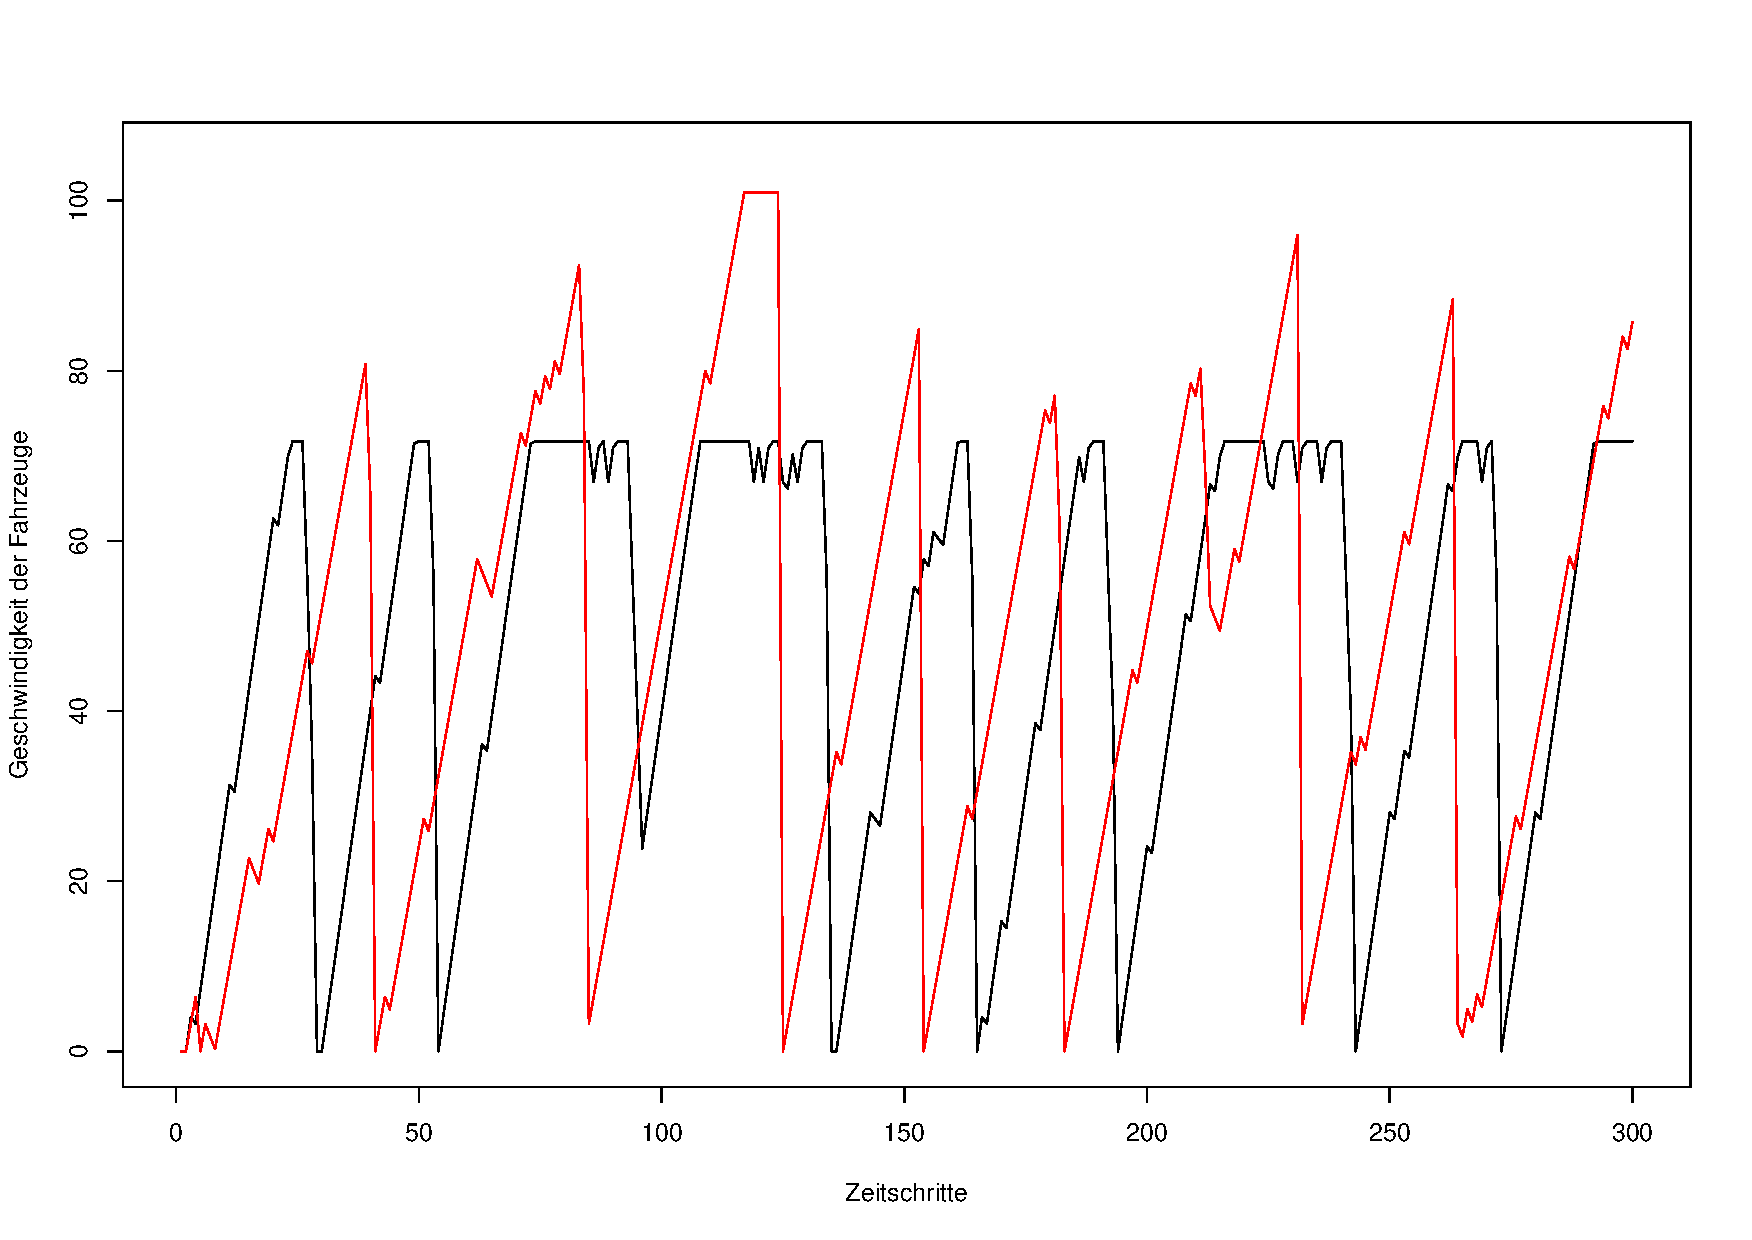
\includegraphics[width=0.3\textwidth]{speed_run1}\label{figure:run1}}\qquad 
   \subfigure[2. Durchlauf]{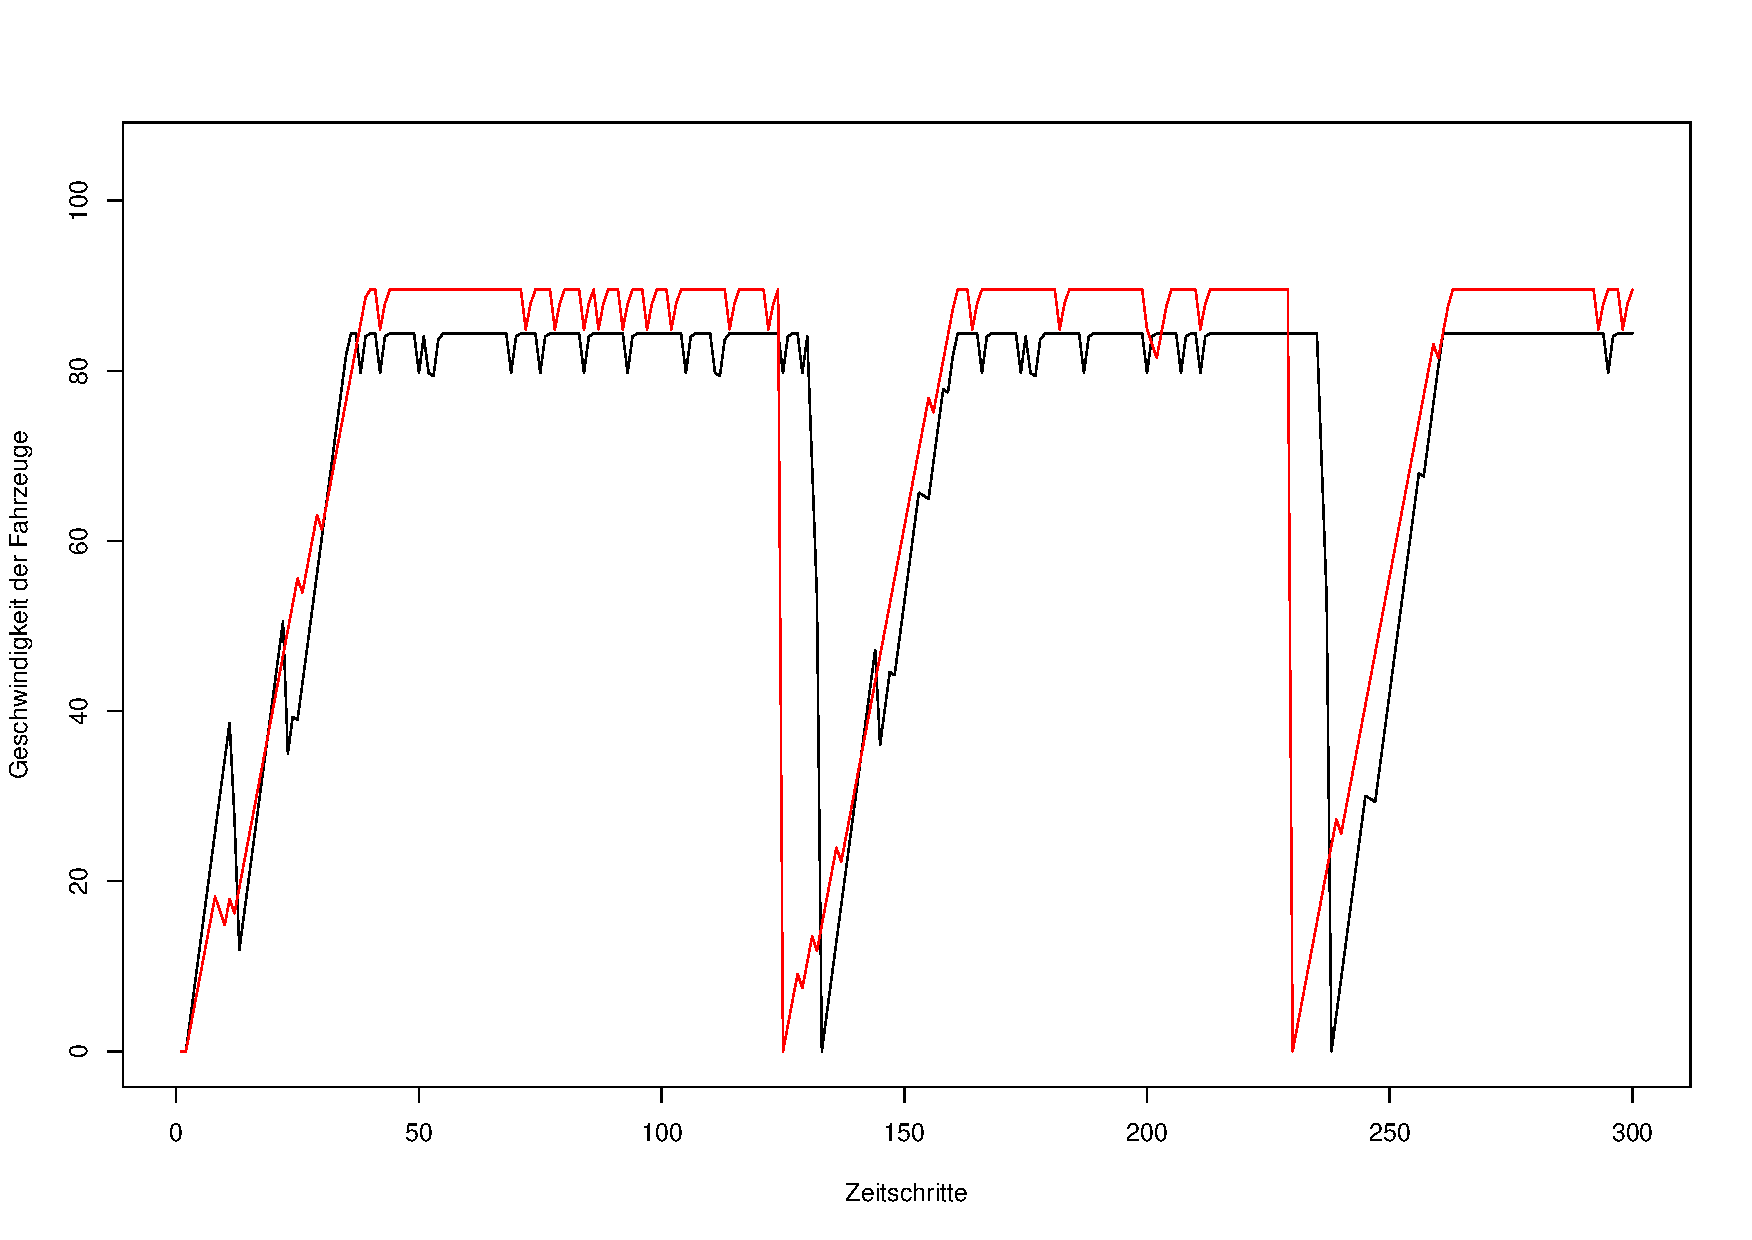
\includegraphics[width=0.3\textwidth]{speed_run2}\label{figure:run2}}\qquad 
   \subfigure[3. Durchlauf]{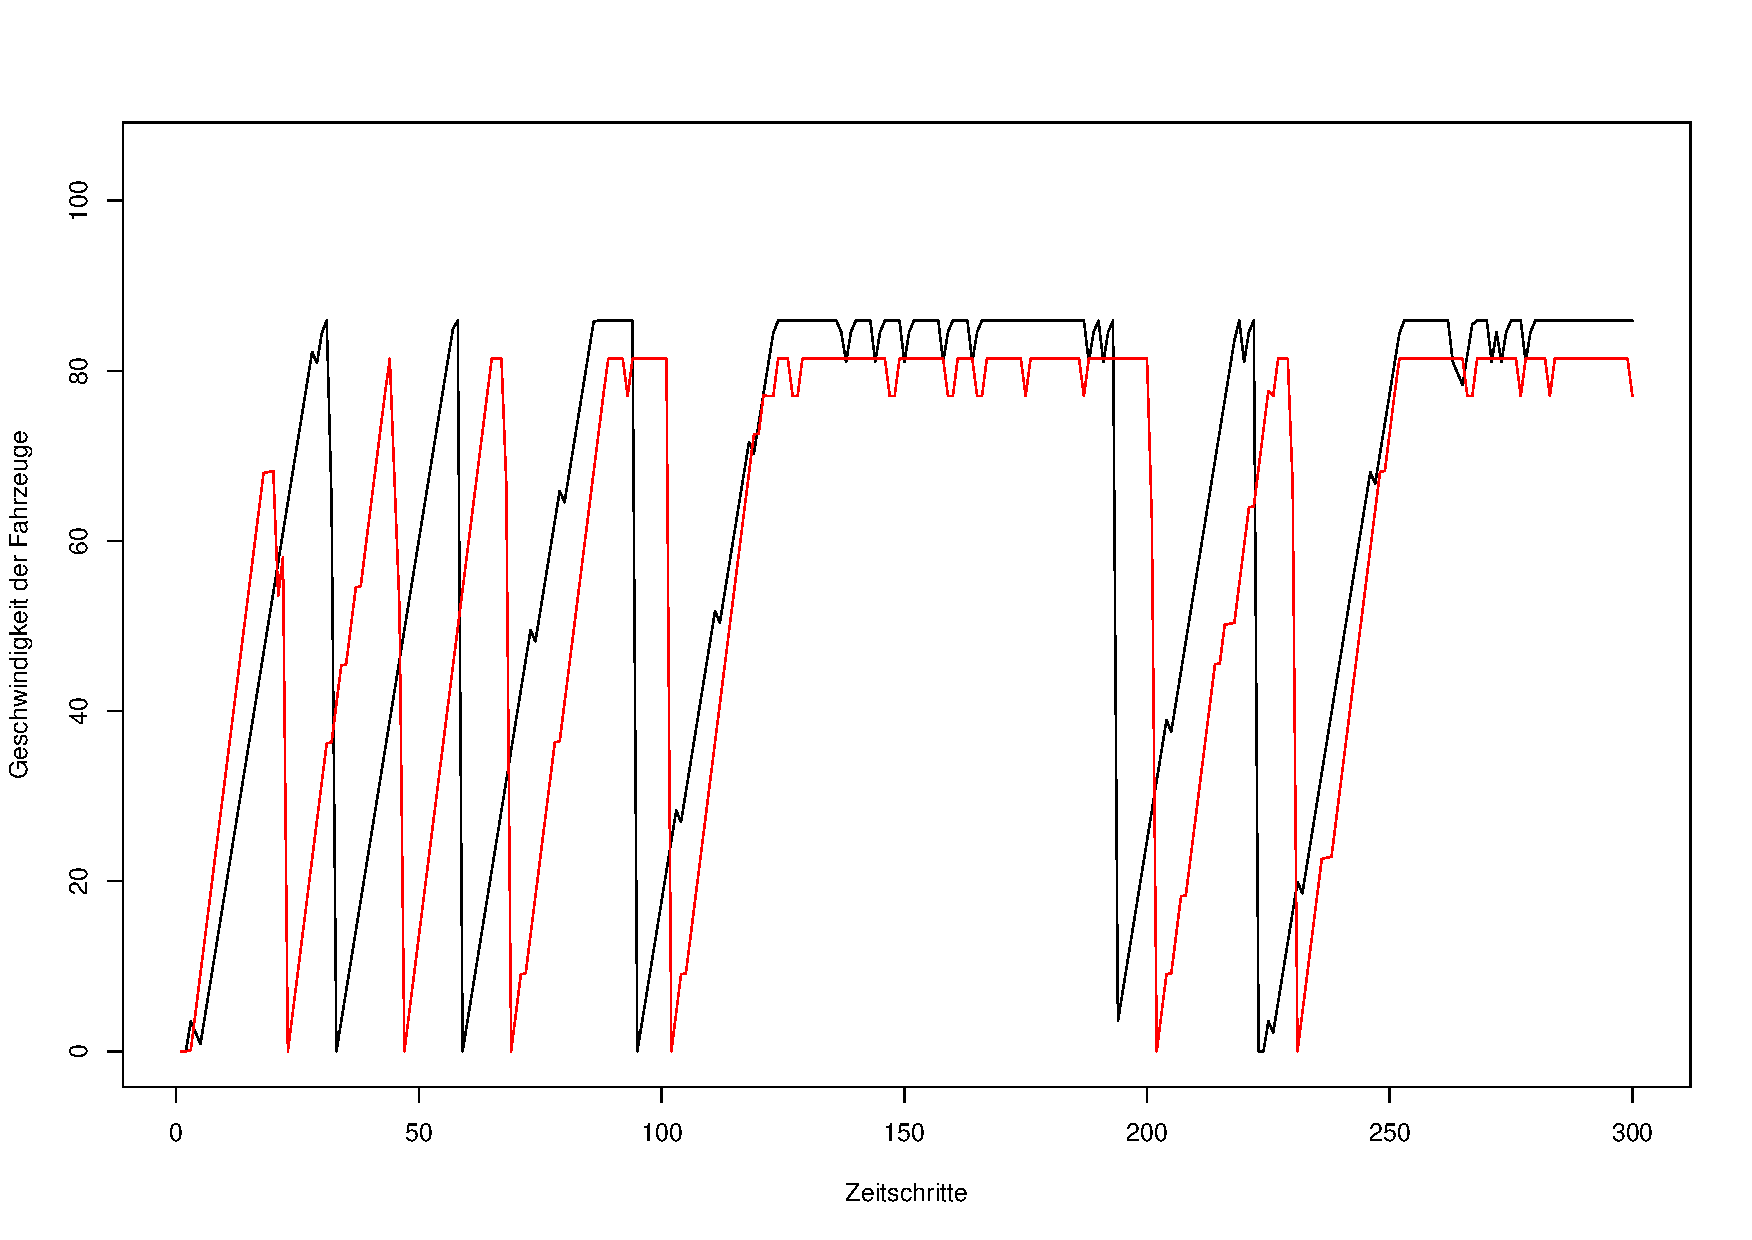
\includegraphics[width=0.3\textwidth]{speed_run3}\label{figure:run3}}
  \caption{Simulationen mit Zellgröße 7,5 m und Zeitschrittlänge 0,1 min} 
  \label{figure:run1-3}
\end{figure}

In allen drei Kurvenverläufen in \cref{figure:run1-3} sind mehrfach Reduktionen der Geschwindigkeit auf Null zu sehen. 
Dies zeigt, dass an diesen Stellen eine Kollision stattgefunden hat. Das Kollisionsereignis wird vom Simulationstool ausgelöst, wenn ein Fahrzeug nicht in der Lage wäre, im nächsten Zeitschritt die für seine Geschwindigkeit entsprechende Streckenlänge zurückzulegen.

Die Zeitschrittlänge von 0,1 Minuten, was sechs Sekunden entspricht, ist nicht ausreichend, um Geschwindigkeit in ausreichendem Maße abzubauen, um genug Abstand vom Vordermann einzuhalten.

Auf die Ausführung von Durchgängen mit dieser Zeitschrittgröße und kleinerer Zellgröße wurde verzichtet.

\begin{figure}[hptb]
  \centering 
   \subfigure[1. Durchlauf]{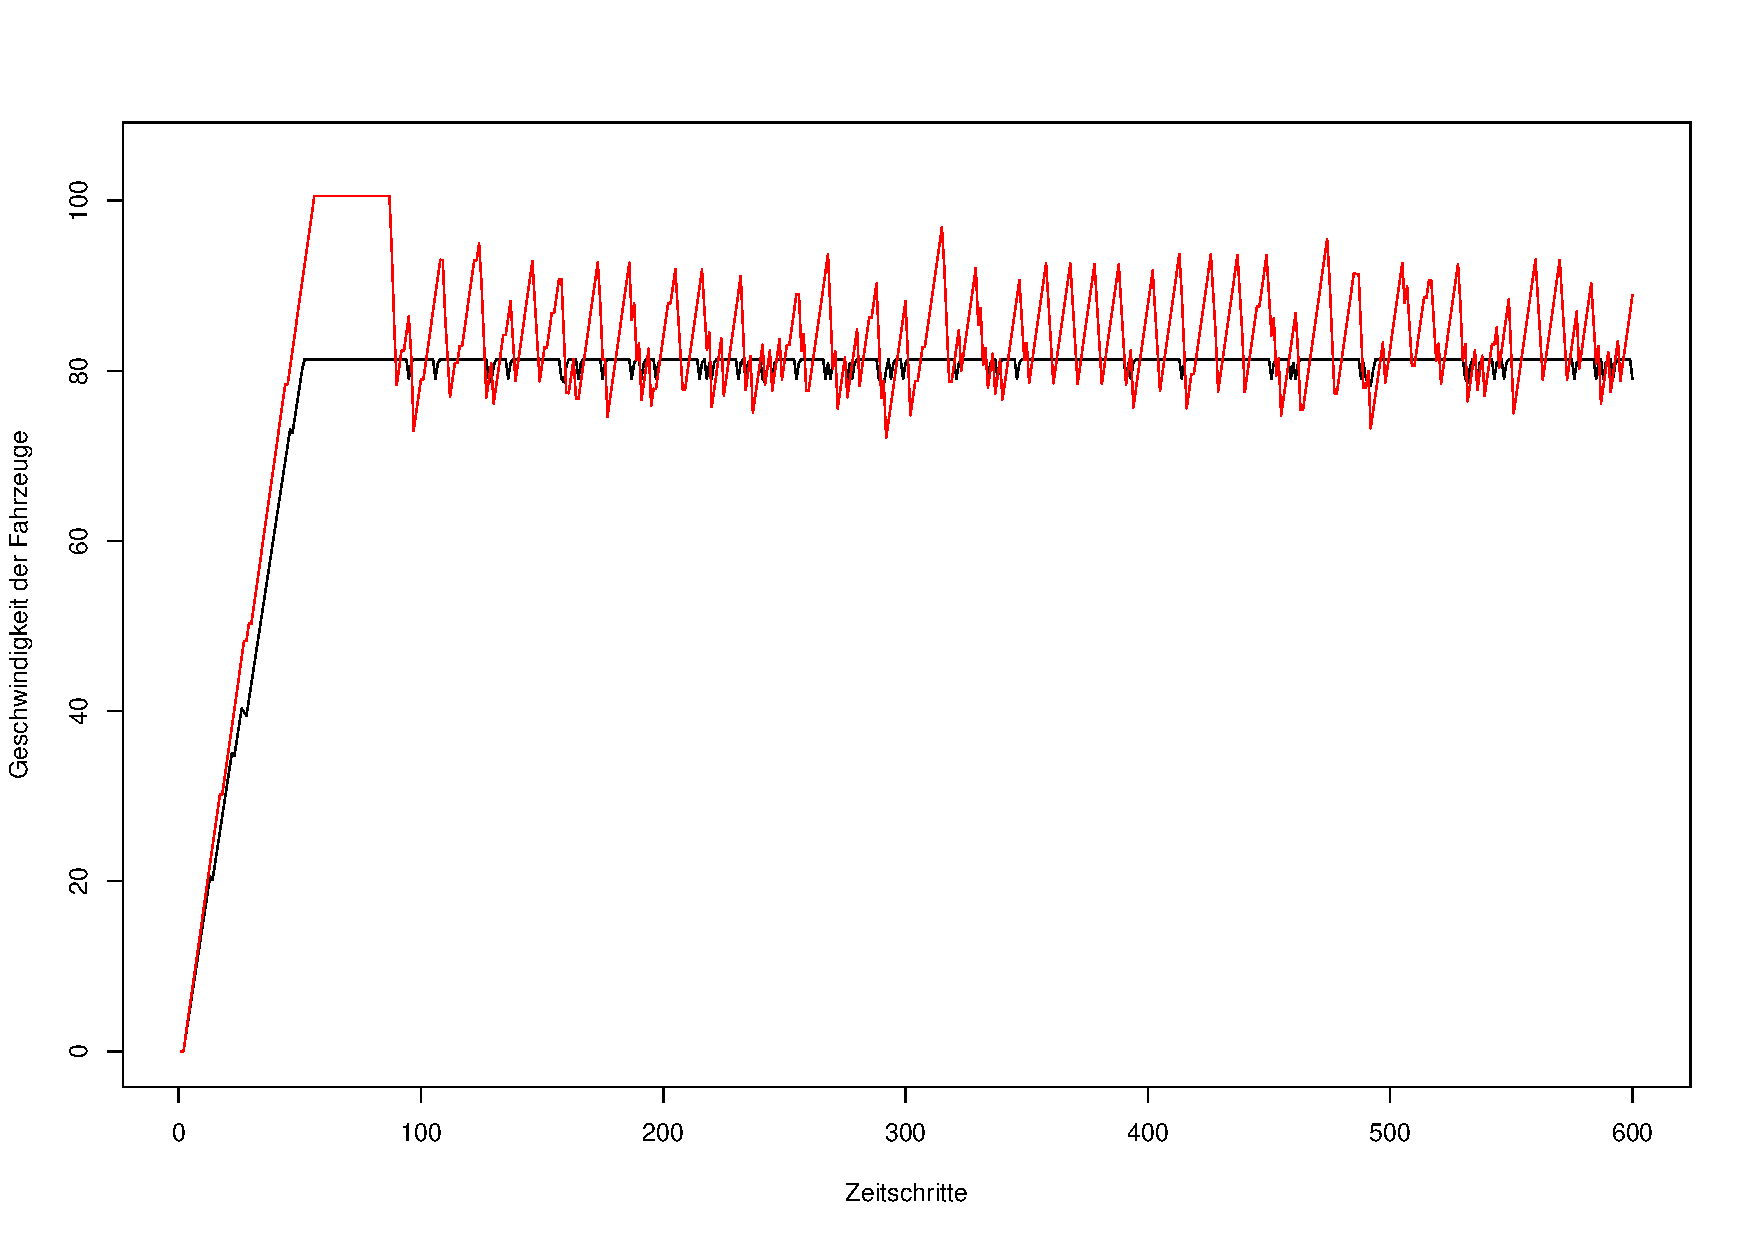
\includegraphics[width=0.3\textwidth]{speed_run4}\label{figure:run4}}\qquad 
   \subfigure[2. Durchlauf]{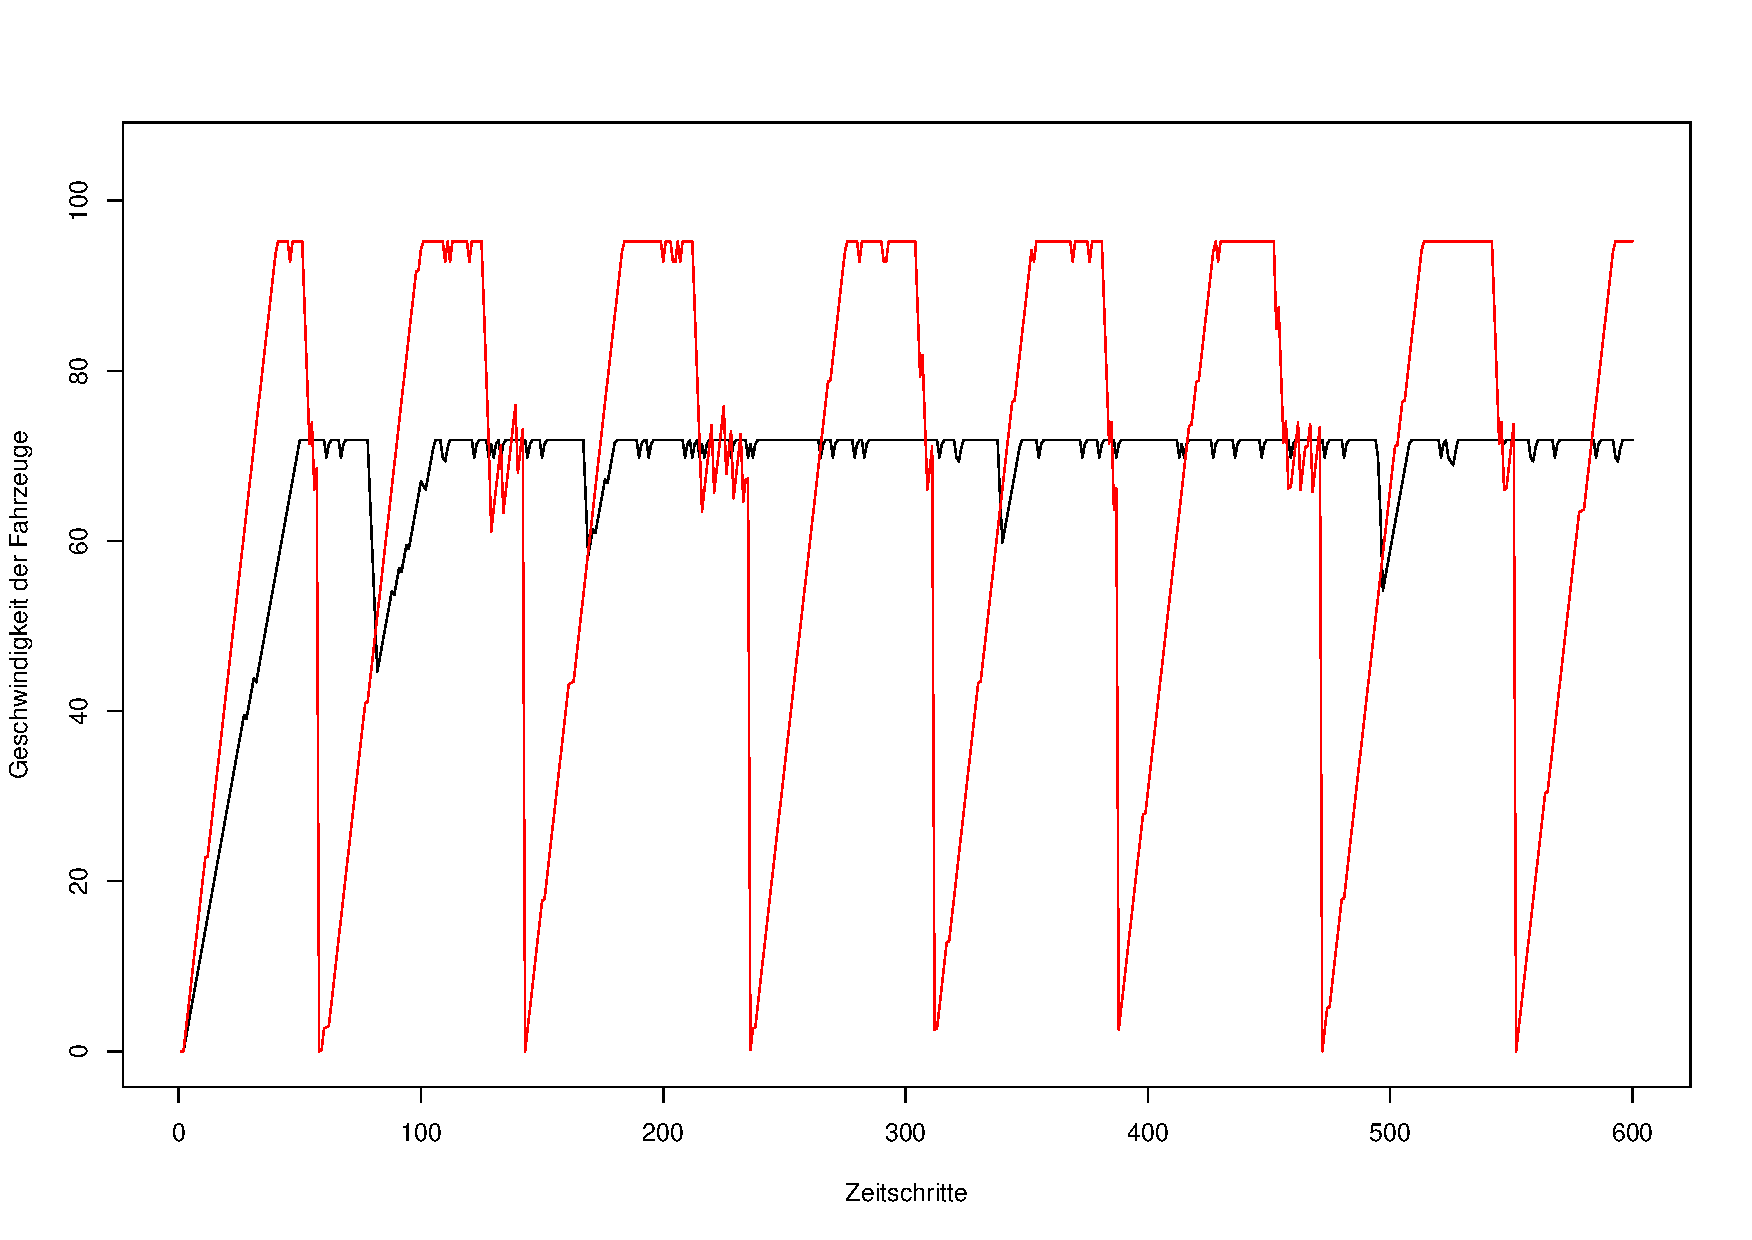
\includegraphics[width=0.3\textwidth]{speed_run5}\label{figure:run5}}\qquad 
   \subfigure[3. Durchlauf]{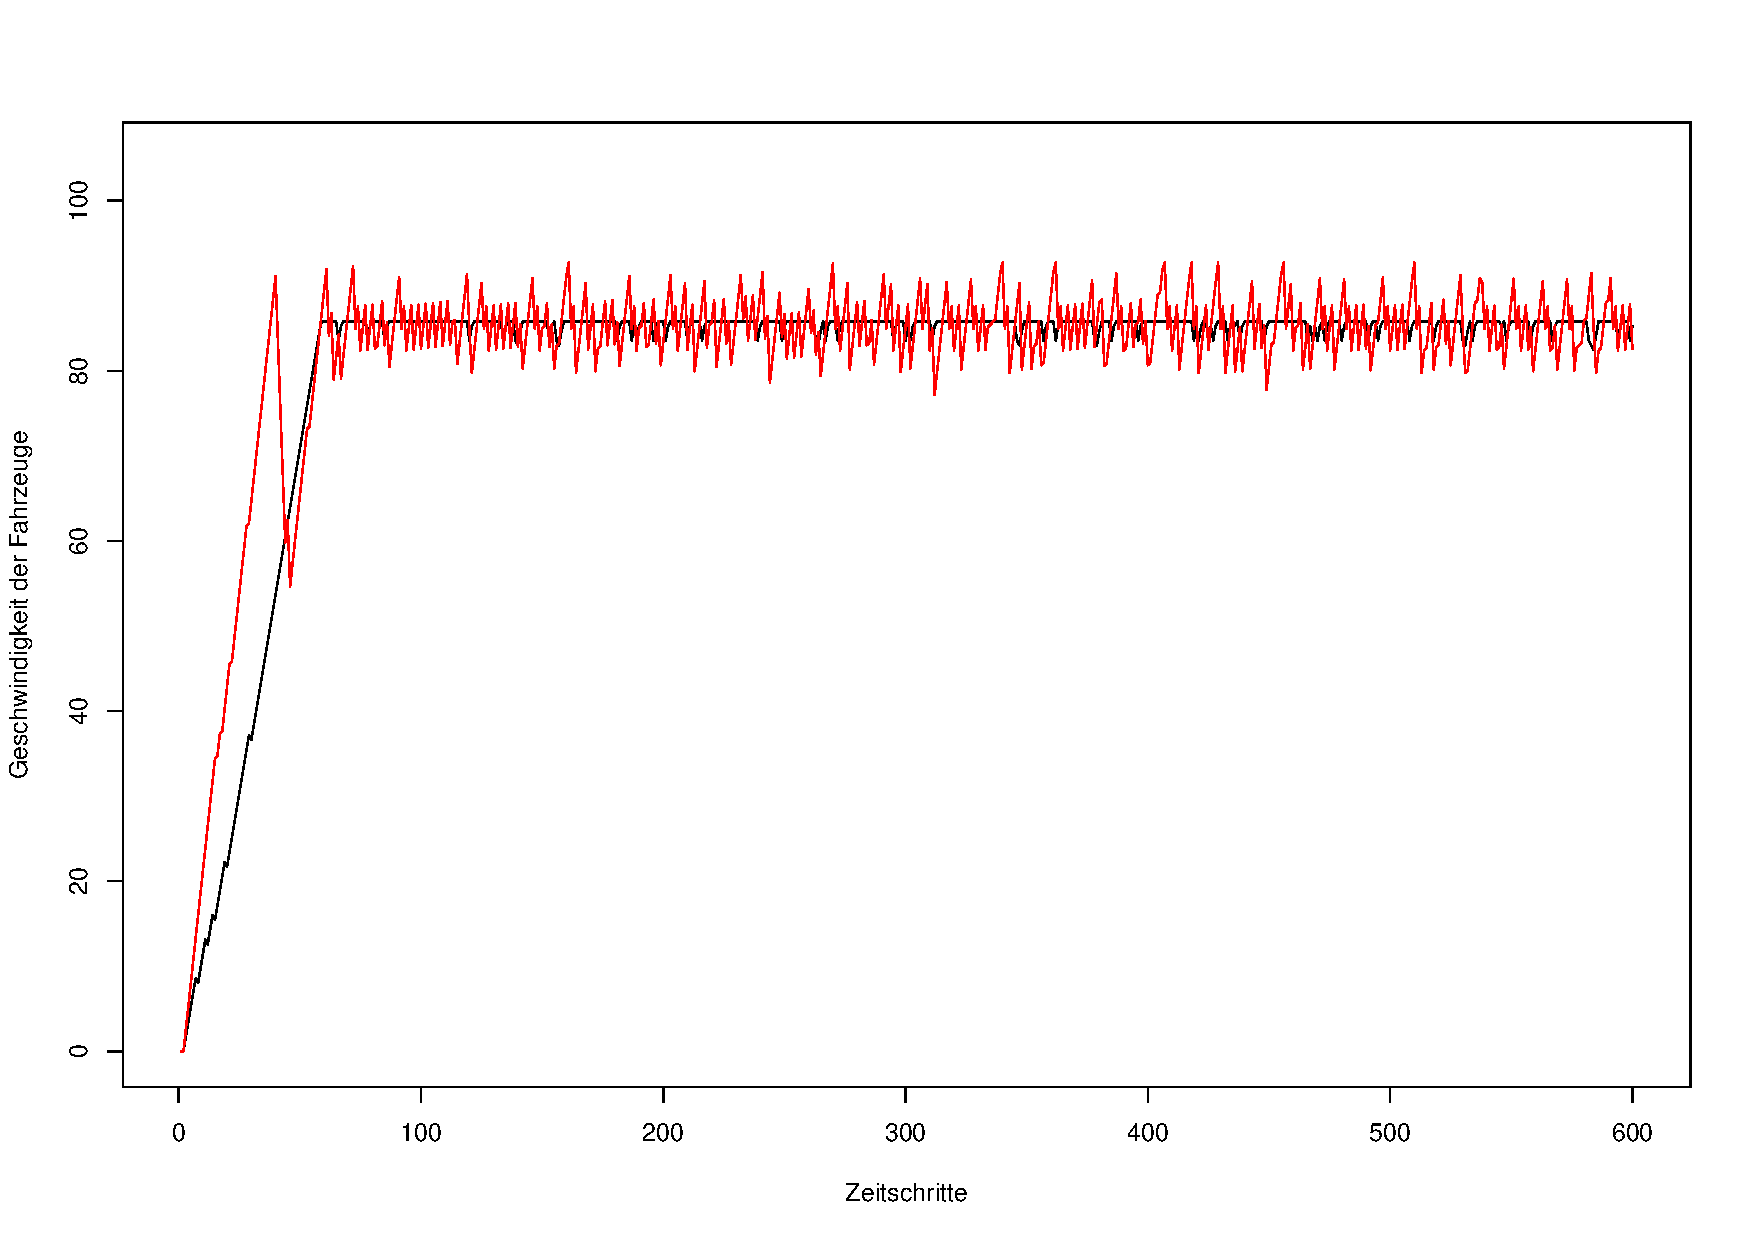
\includegraphics[width=0.3\textwidth]{speed_run6}\label{figure:run6}}
  \caption{Simulationen mit Zellgröße 7,5 m und Zeitschrittlänge 0,05 min} 
  \label{figure:run4-6}
\end{figure}

Die Verläufe der Kurven in \cref{figure:run4-6} zeigen in zwei von drei Fällen, dass sich die Geschwindigkeit des auffahrenden Fahrzeuges um die des langsameren Fahrzeuges einpendelt.

Im Plot des zweiten Durchlaufes ist zu sehen, dass auch in dieser Konstellation Kollisionen stattgefunden haben.
Die Geschwindigkeit des langsameren Fahrzeuges lag in diesem Durchlauf im Vergleich zu den anderen beiden um einiges niedriger.

\begin{figure}[hptb]
  \centering 
   \subfigure[1. Durchlauf]{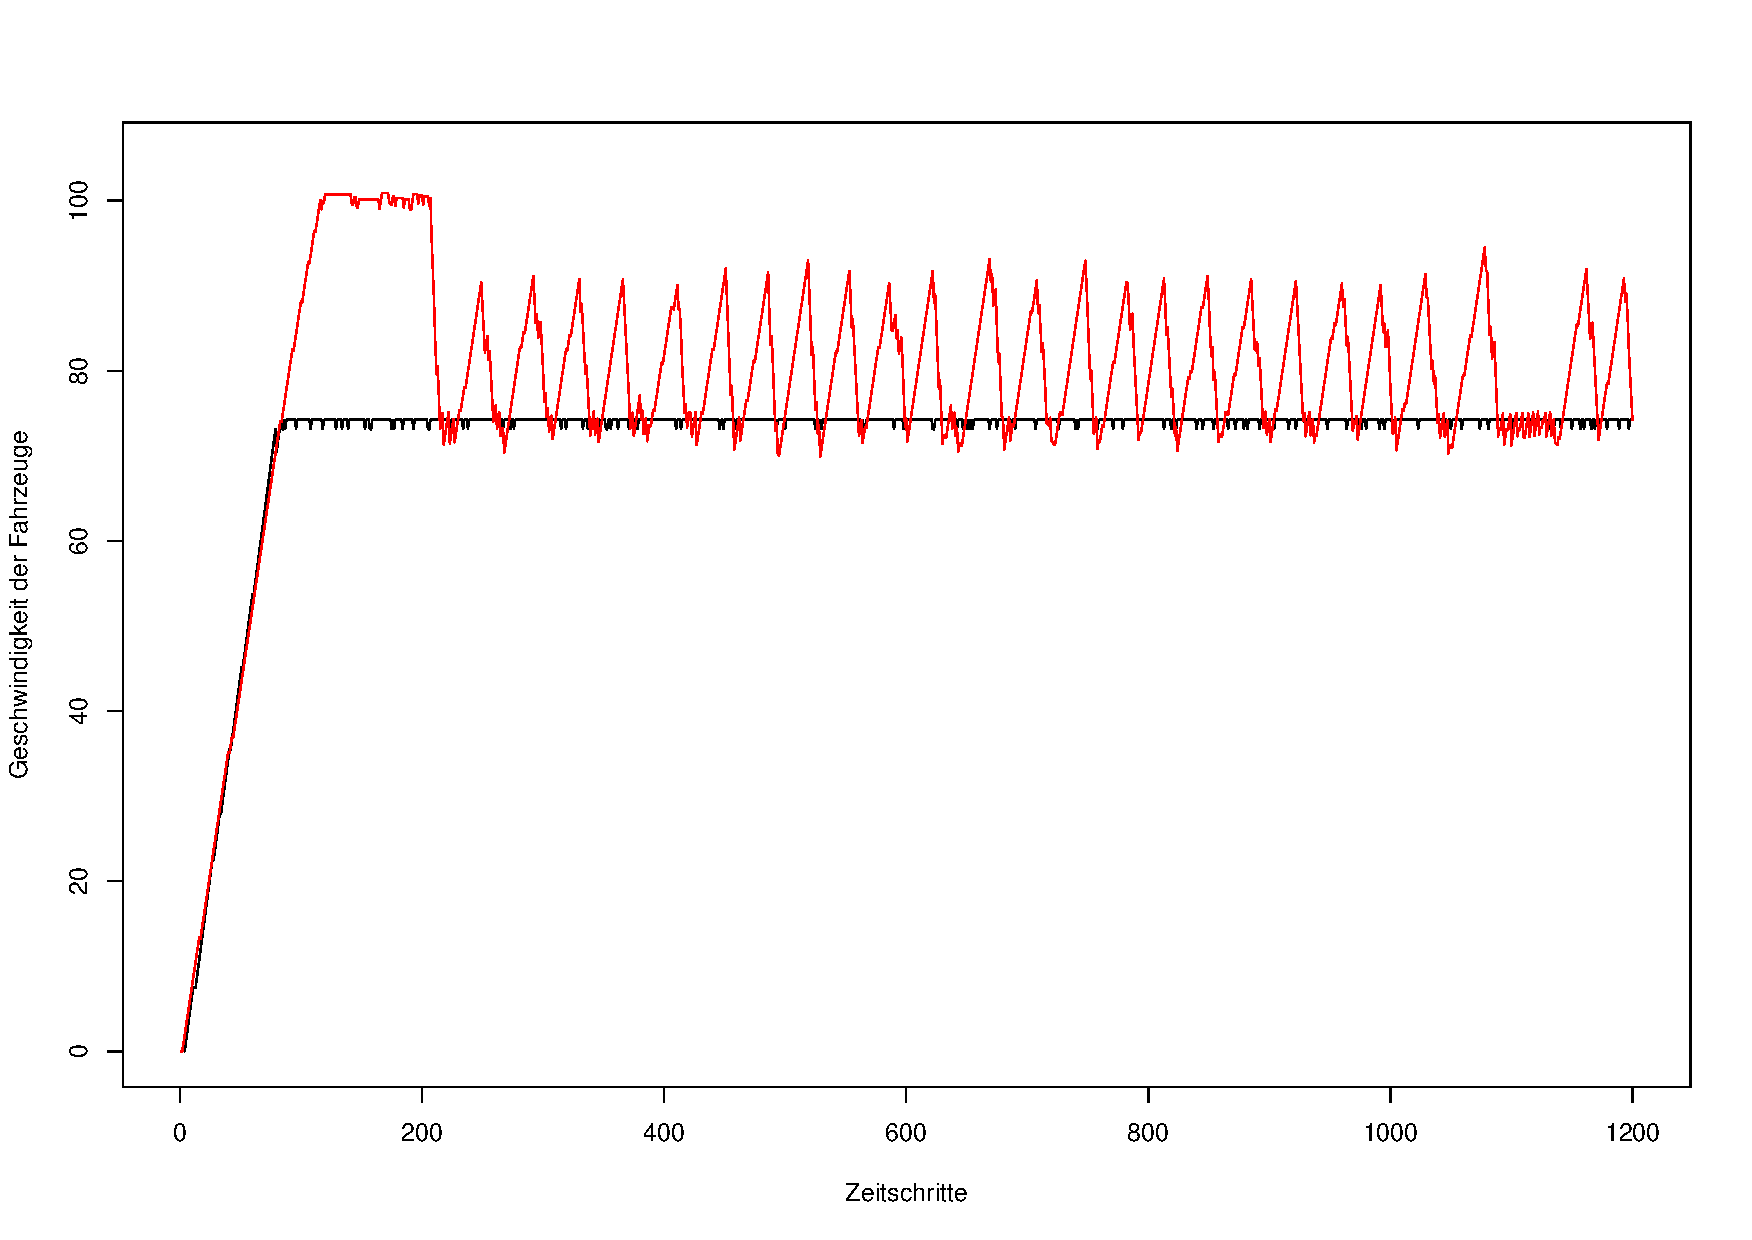
\includegraphics[width=0.3\textwidth]{speed_run7}\label{figure:run7}}\qquad 
   \subfigure[2. Durchlauf]{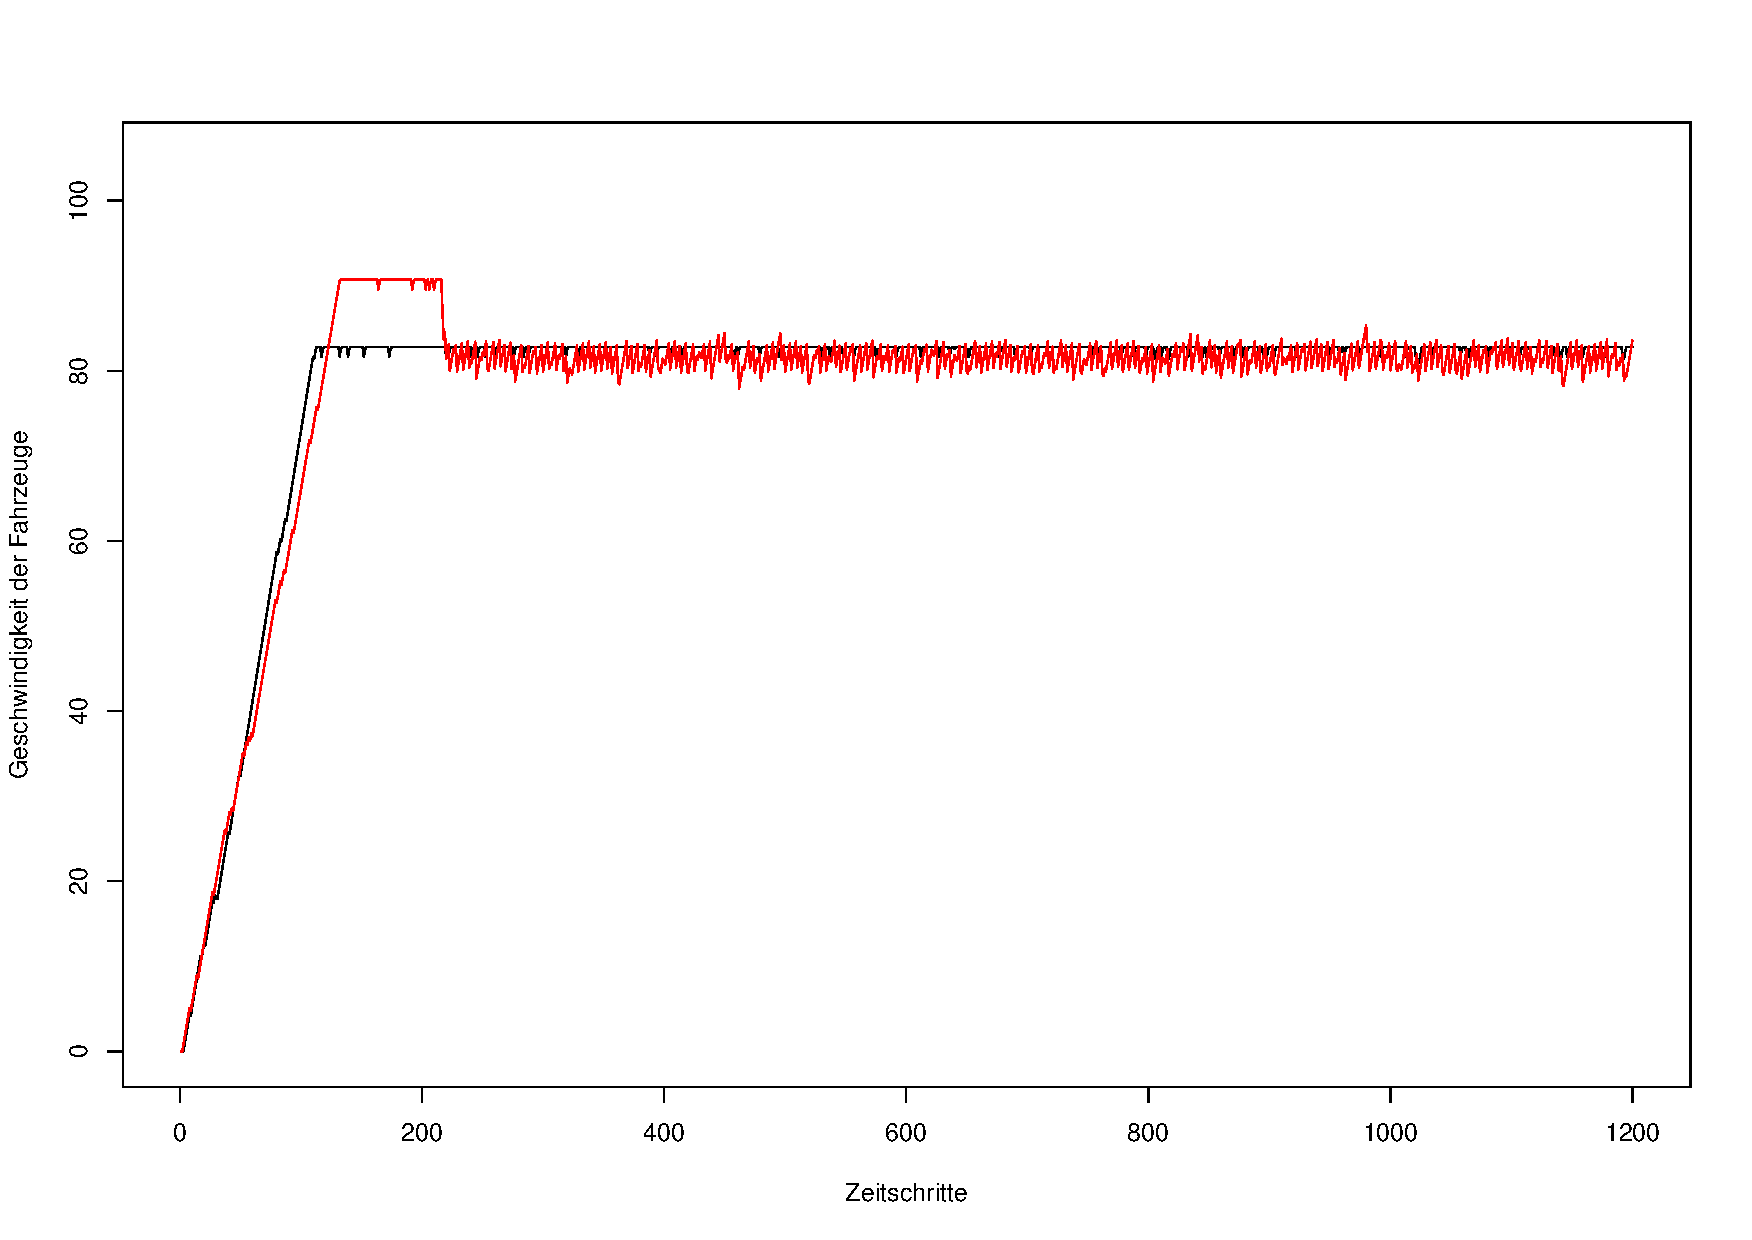
\includegraphics[width=0.3\textwidth]{speed_run8}\label{figure:run8}}\qquad 
   \subfigure[3. Durchlauf]{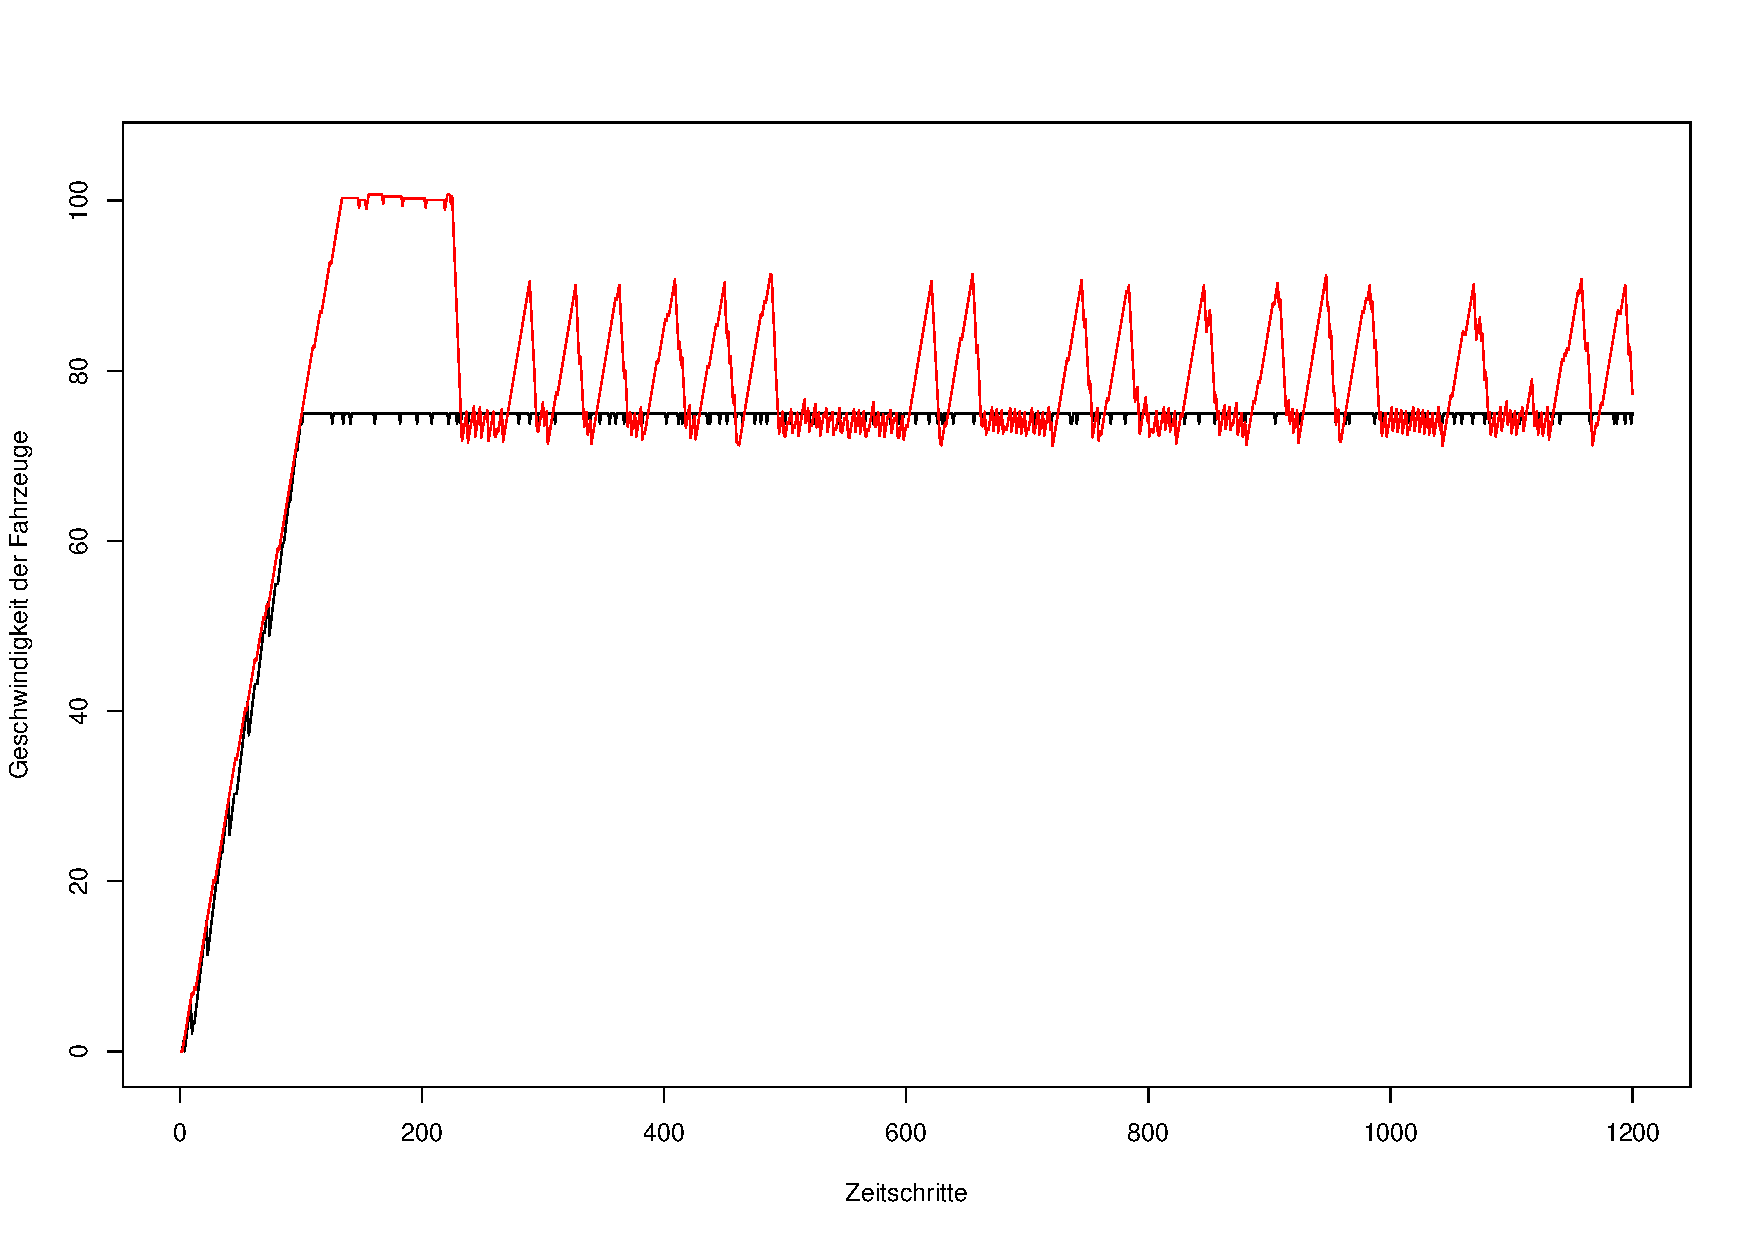
\includegraphics[width=0.3\textwidth]{speed_run9}\label{figure:run9}}
  \caption{Simulationen mit Zellgröße 7,5 m und Zeitschrittlänge 0,025 min} 
  \label{figure:run7-9}
\end{figure}

Die Geschwindigkeitskurve des schnelleren Fahrzeugs weist in \cref{figure:run7} ein sägezahnähnliches Muster auf.
Dies resultiert aus den, im Vergleich zu den herbeigeführten Geschwindigkeitszuwächsen, großen Zellen.
Ein Geschwindigkeitsunterschied von zehn bis 15 km/h reicht bei entsprechend zugrunde liegender Ausgangsgeschwindigkeit nicht aus, eine Verkürzung des Abstands herbeizuführen.
Da sich die Abbrems- und Beschleunigungsmanöver identisch wiederholen, kommt es zu dieser Musterbildung.

Das Plot in \cref{figure:run8} zeigt ein Einordnen hinter dem langsameren Fahrzeug und die Beibehaltung dessen Geschwindigkeit.
Das in \cref{figure:run9} ist nahezu eine Mischform aus den ersten beiden Kurven.


\subsubsection{Zellgröße 5,0 m}

\begin{figure}[hptb]
  \centering 
   \subfigure[1. Durchlauf]{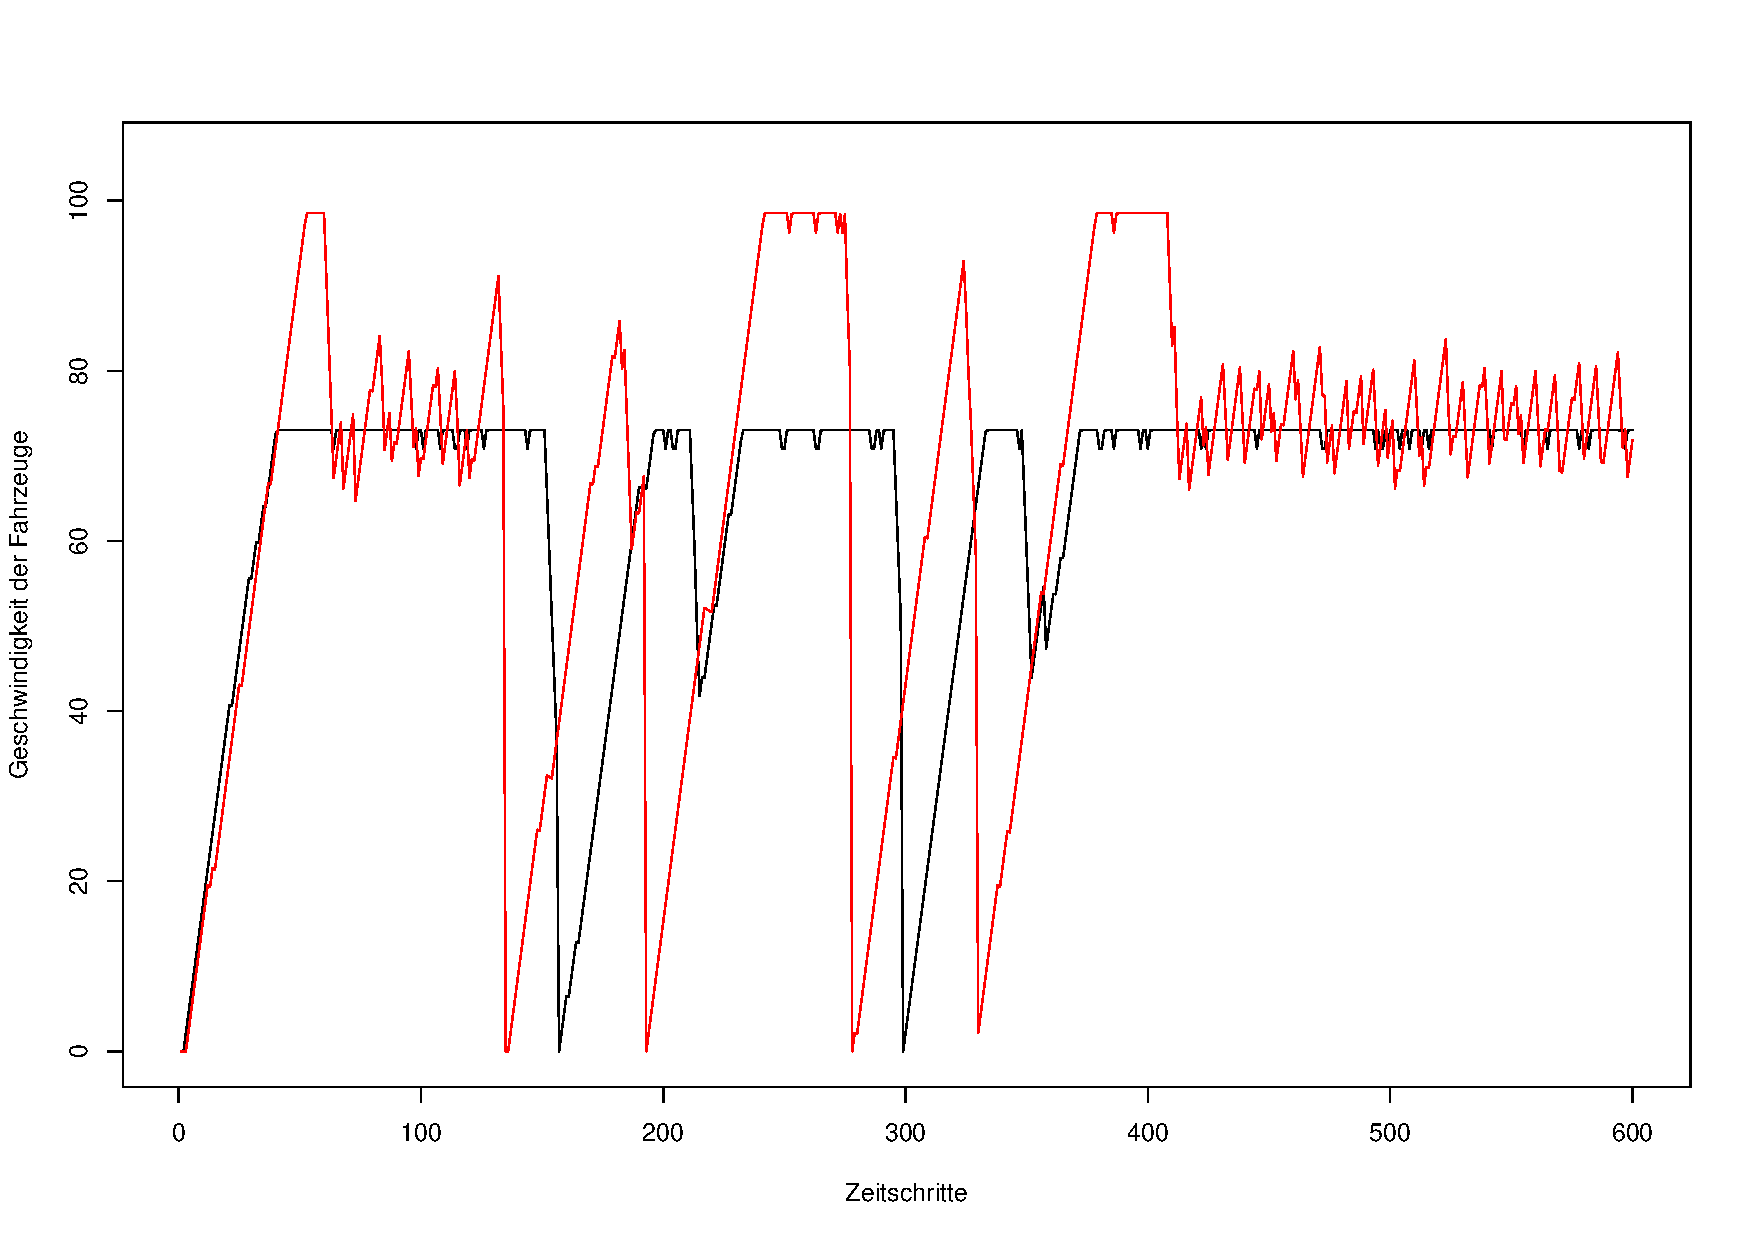
\includegraphics[width=0.3\textwidth]{speed_run14}\label{figure:run14}}\qquad 
   \subfigure[2. Durchlauf]{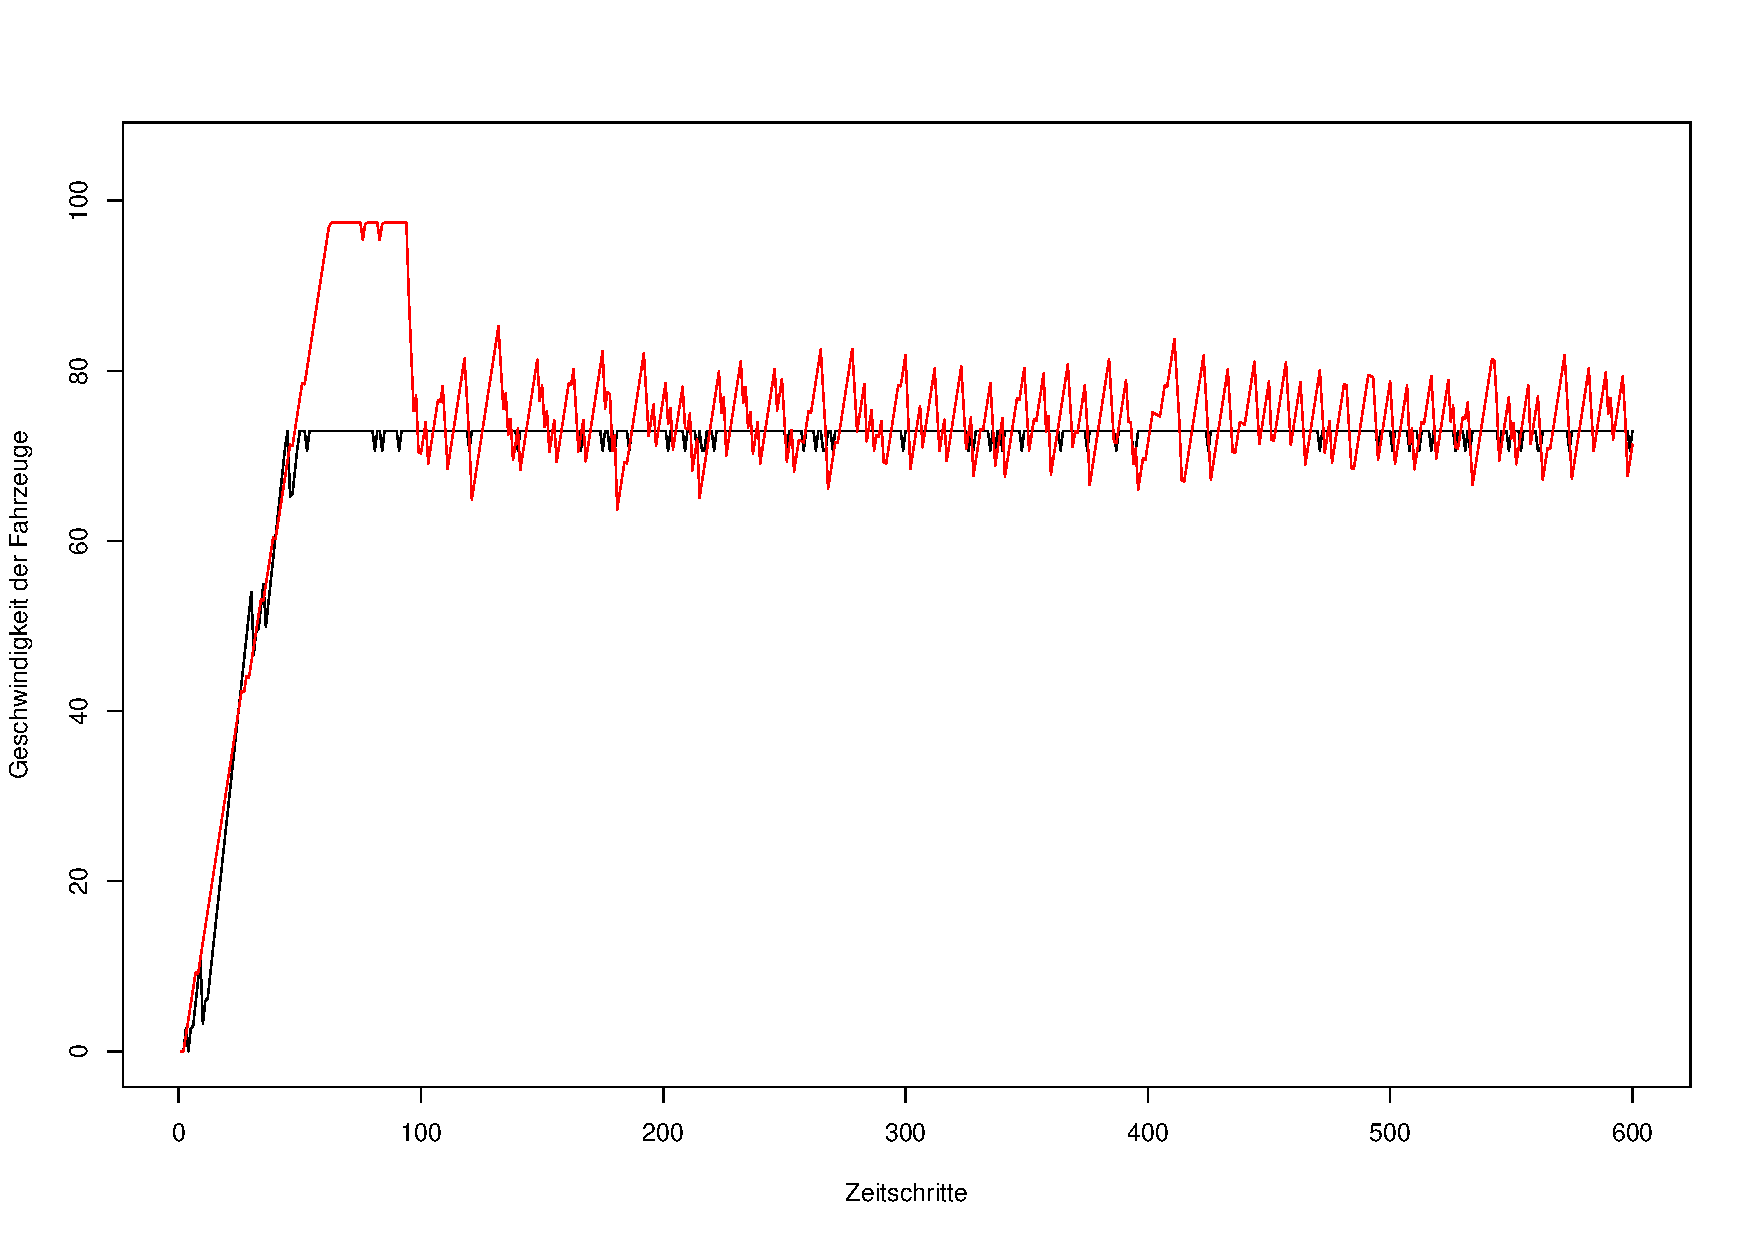
\includegraphics[width=0.3\textwidth]{speed_run15}\label{figure:run15}}\qquad 
   \subfigure[3. Durchlauf]{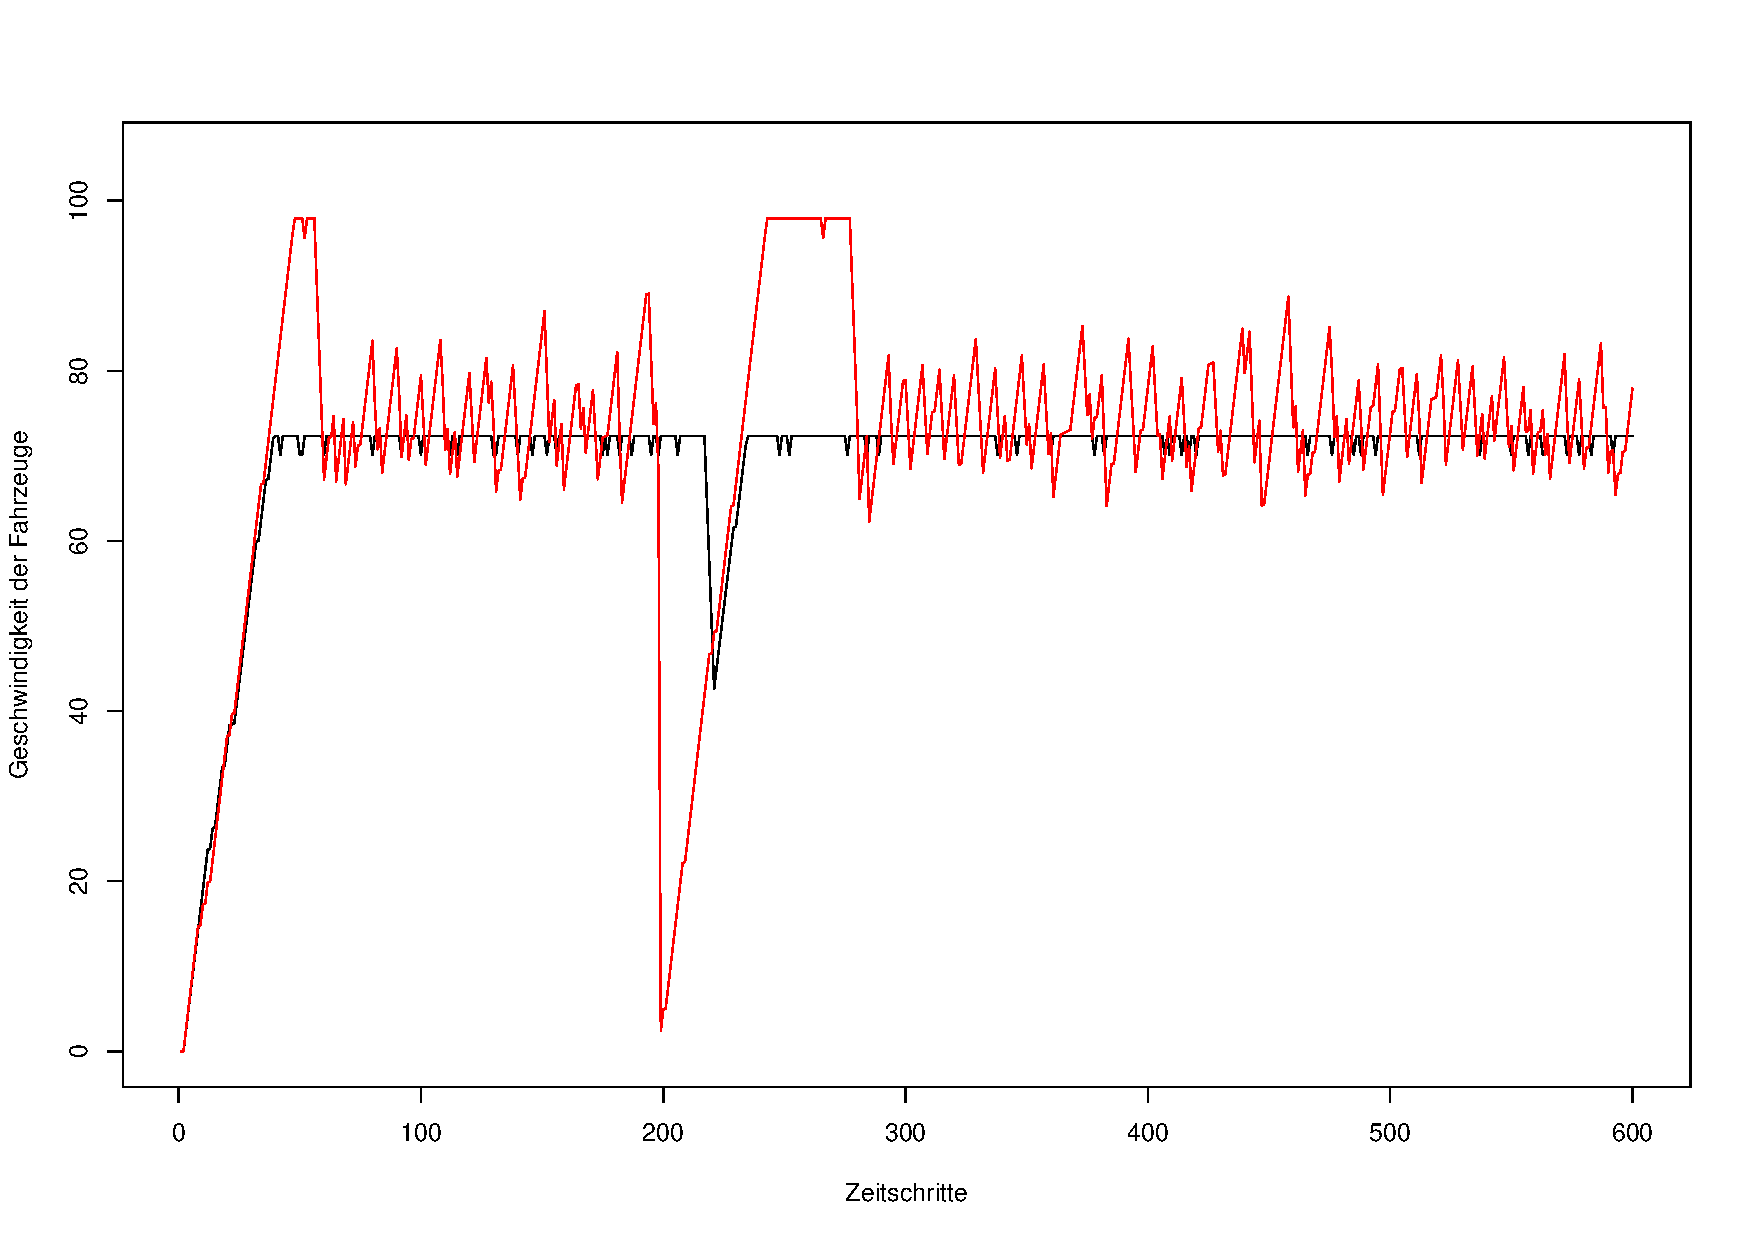
\includegraphics[width=0.3\textwidth]{speed_run16}\label{figure:run16}}
  \caption{Simulationen mit Zellgröße 5,0 m und Zeitschrittlänge 0,05 min} 
  \label{figure:run14-16}
\end{figure}

Die Diagramme in \cref{figure:run14-16} zeigen wiederholt, dass der Abstand, der für den Bremsvorgang zur Verfügung steht, mit einem recht langen Zeitraum zwischen den Zeitschritten, nicht ausreicht.

Allerdings ist im ersten und im dritten Durchlauf zu erkennen, dass das langsamere Fahrzeug, ohne dass es zu einer Kollision kommen muss, für das gerade beschleunigende Fahrzeug abbremsen konnte. 

\begin{figure}[hptb]
  \centering 
   \subfigure[1. Durchlauf]{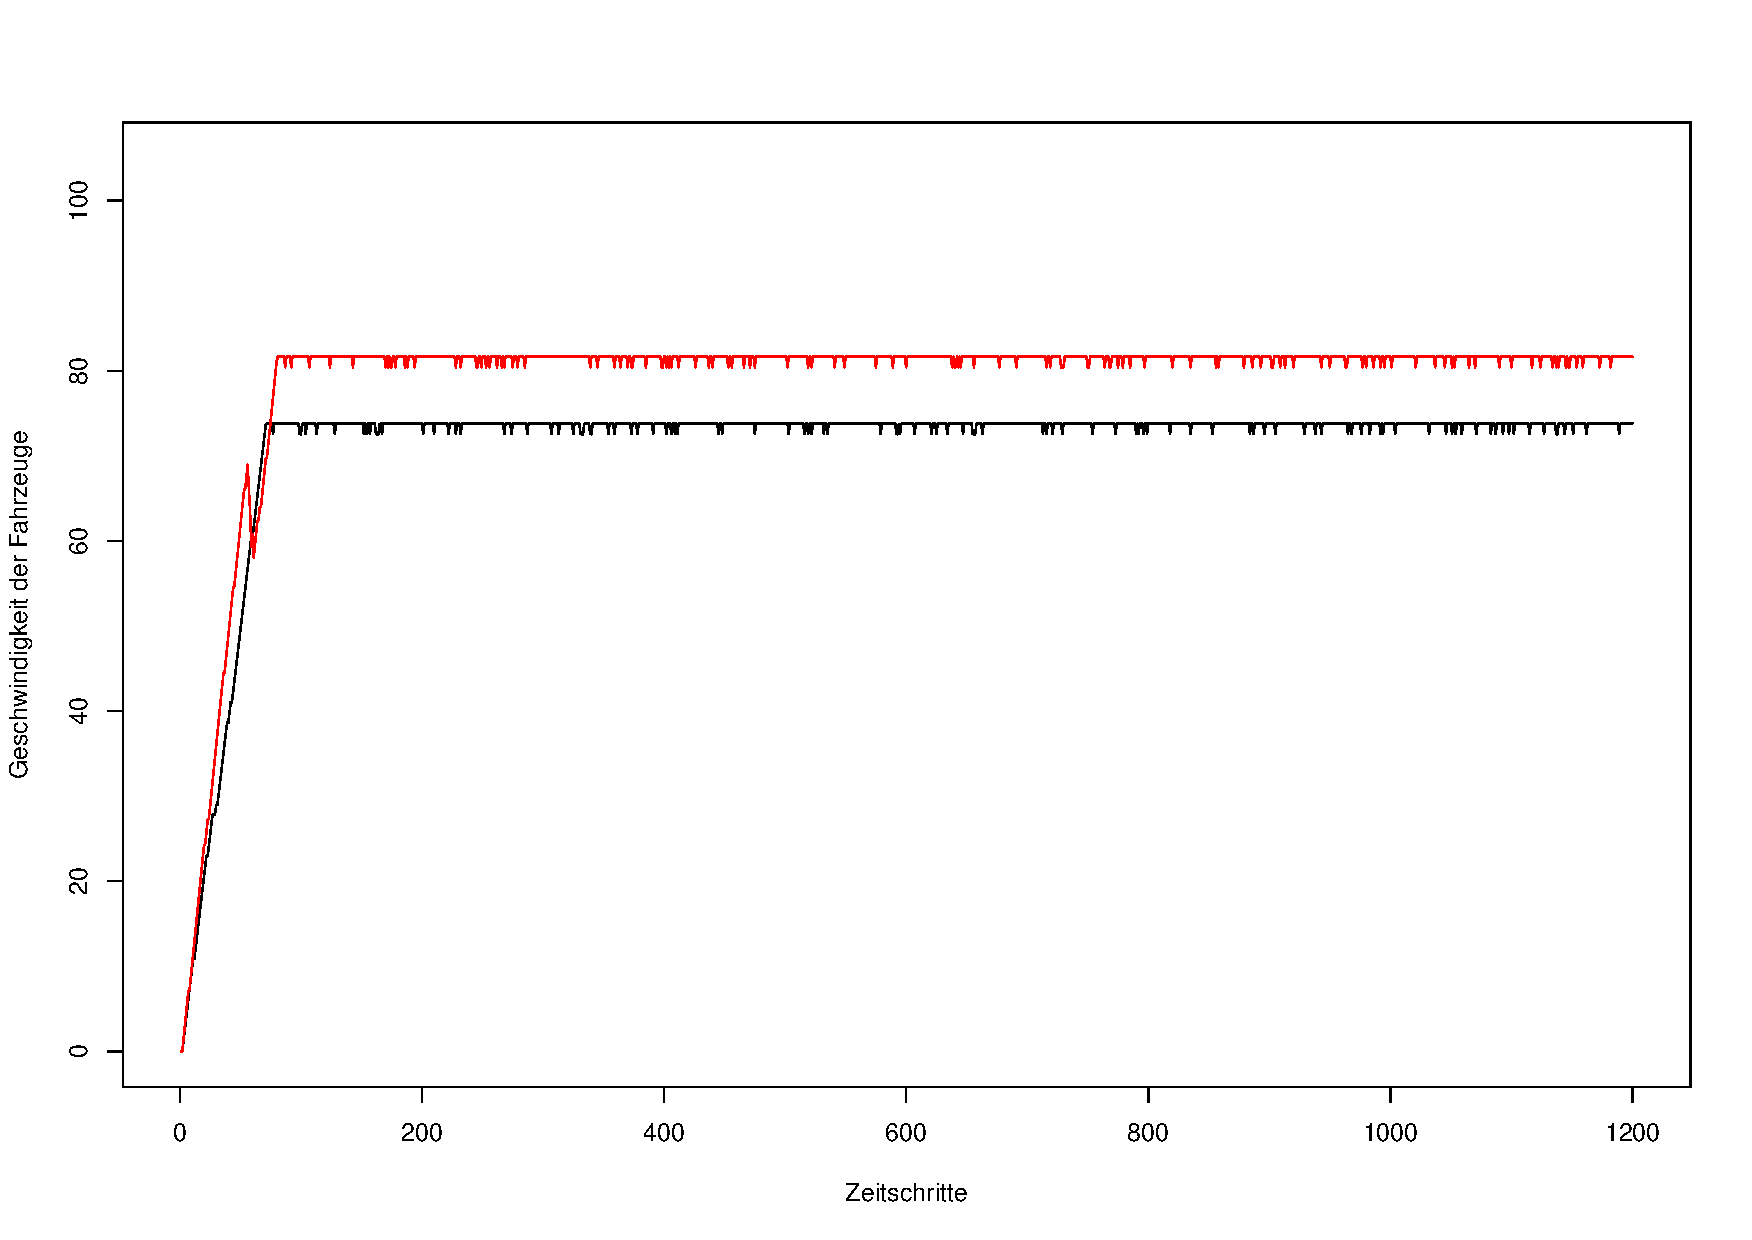
\includegraphics[width=0.3\textwidth]{speed_run17}\label{figure:run17}}\qquad 
   \subfigure[2. Durchlauf]{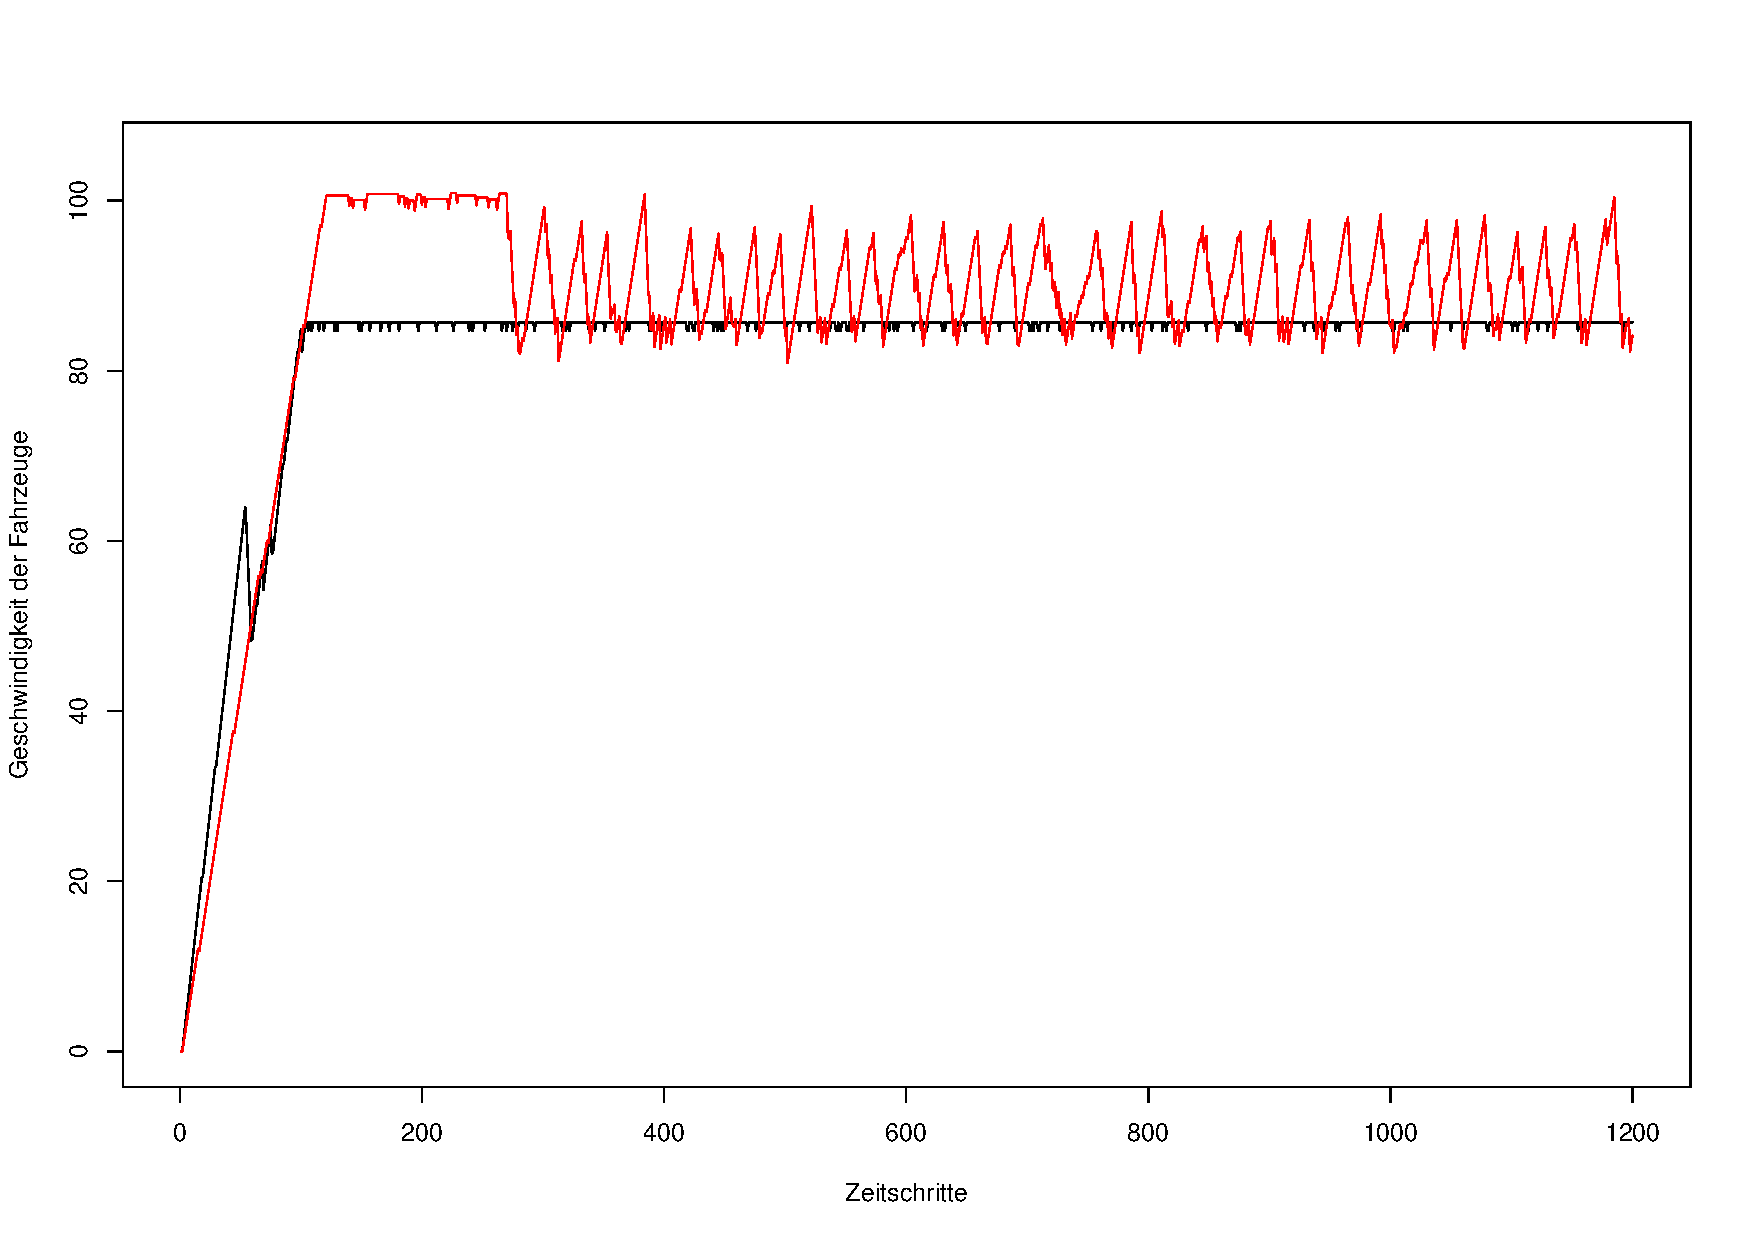
\includegraphics[width=0.3\textwidth]{speed_run18}\label{figure:run18}}\qquad 
   \subfigure[3. Durchlauf]{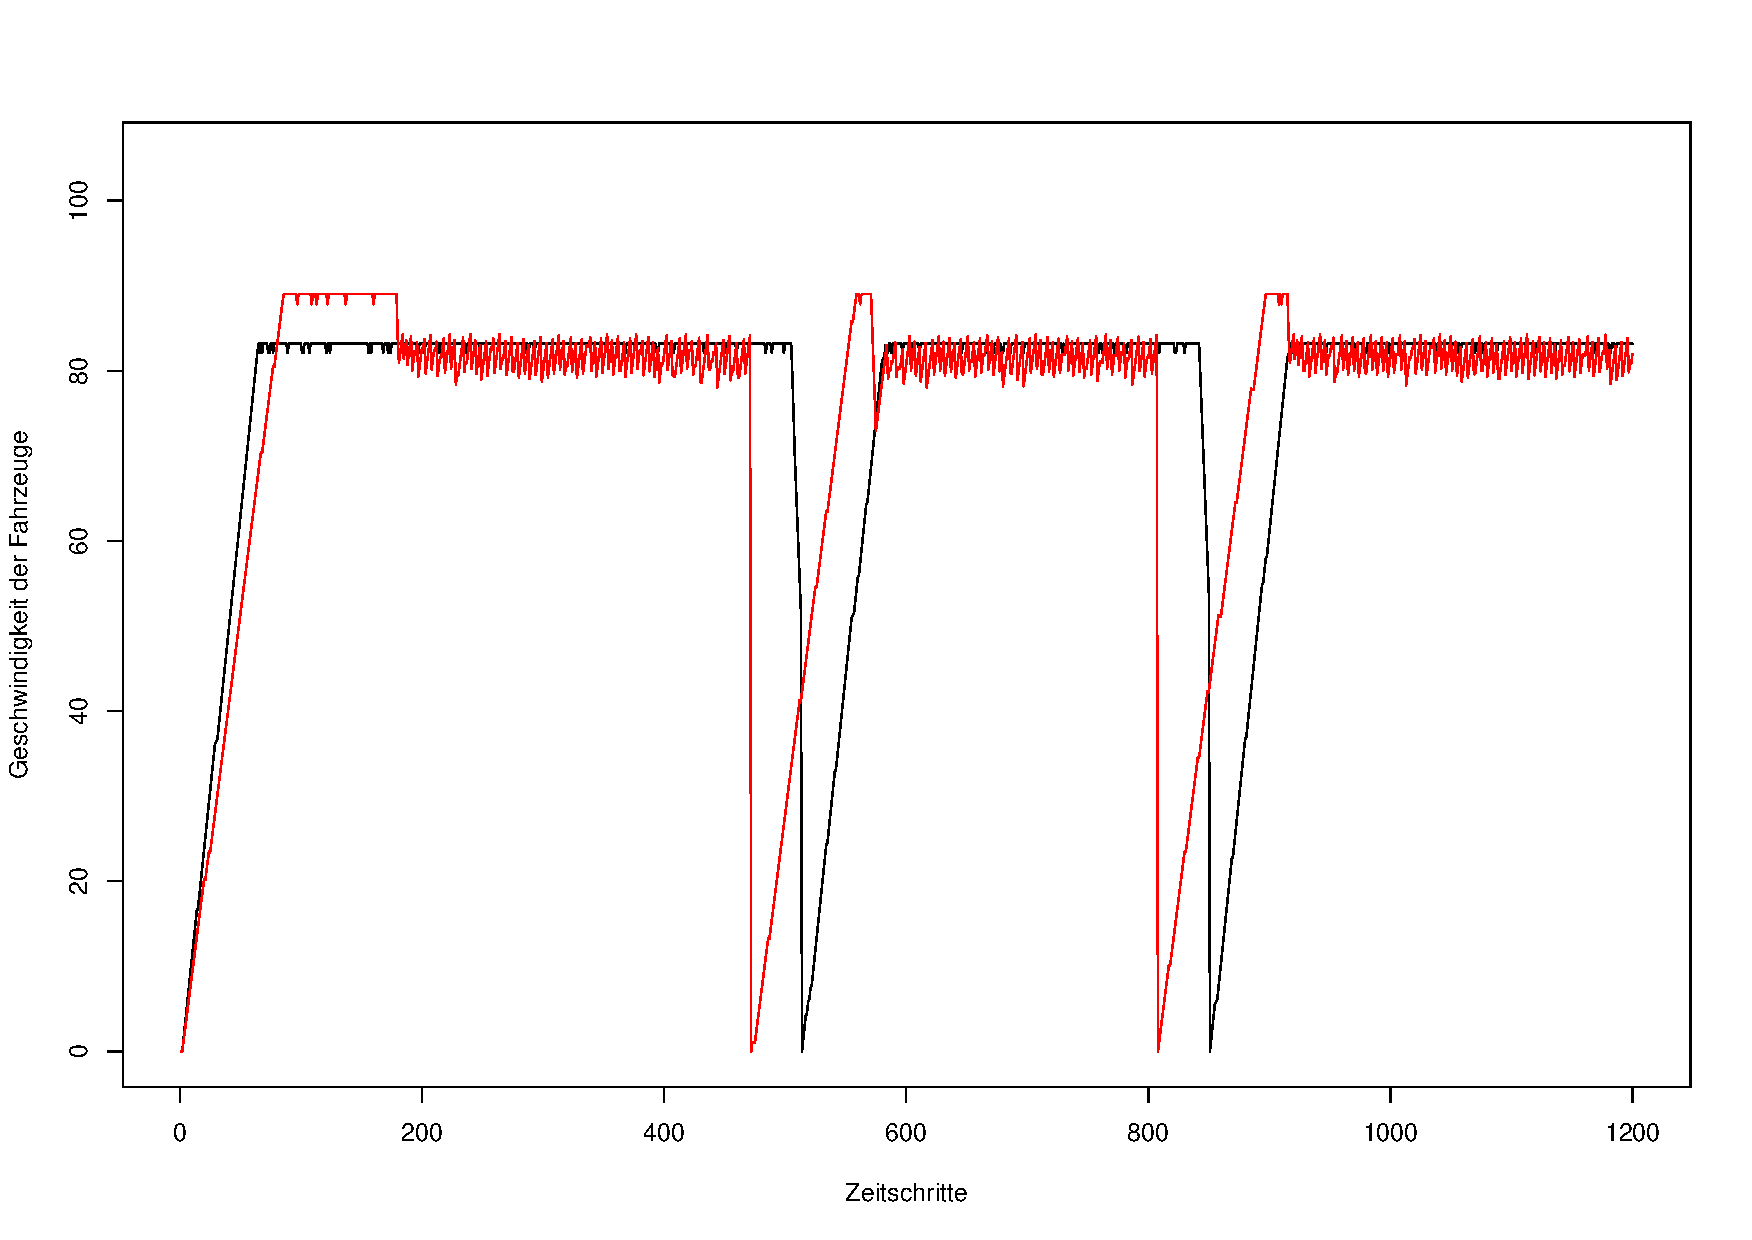
\includegraphics[width=0.3\textwidth]{speed_run19}\label{figure:run19}}
  \caption{Simulationen mit Zellgröße 5,0 m und Zeitschrittlänge 0,025 min} 
  \label{figure:run17-19}
\end{figure}

Die drei Durchläufe mit einer Zeitschrittlänge von 0,025 min ergaben ein uneinheitliches Bild.
In \cref{figure:run17} konnte das schnellere Fahrzeug wieder mit höherer Geschwindigkeit hinter dem langsameren herfahren, scheinbar ohne dass ein Raumgewinn passierte, der zu einer Verzögerung geführt hätte.
\\
Evtl. fuhr das schnellere Fahrzeug auch mit seiner max. möglichen Geschwindigkeit und der Geschwindigkeitsunterschied war so gering, das es in der Simulationszeit das langsamere Fahrzeug nicht erreichte.

Der Durchlauf im Diagramm in \cref{figure:run18} zeigt wieder das sägezahnähnliche Muster, wie es mit den größeren Zelldimensionen bereits der Fall war.

Unerwarteterweise kam es im dritten Durchlauf zu je zwei Kollisionen.
Besonders die jeweils auslösende Kollision des ursprünglich schnelleren Fahrzeuges war nicht zu erklären, da der Geschwindigkeitsunterschied in beiden Fällen minimal gewesen war.

Ein weiterer Durchlauf, siehe \cref{figure:run19a}, der einen vergleichbaren Ablauf hervorbrachte, bei dem aber die Ausgabe der Fahrzeugdaten im Kontrollfenster erfolgte, konnte das Verhalten aufklären.
Die Bedingung im Agentenplan waren so formuliert, dass das Folgefahrzeug dem vorausfahrenden folgen konnte, ohne dass ein \enquote{Sicherheitsabstand} gebildet wurde, wenn die Geschwindigkeit jenes Fahrzeuges nicht größer als die des vorausfahrenden Fahrzeuges war. 
\\
Somit genügte, gewisse Geschwindigkeiten vorrausgesetzt, eine kleine Beschleunigung, um im nachfolgenden Zeitschritt die für die Geschwindigkeit erforderliche Wegstrecke nicht mehr umsetzen zu können.

\begin{figure}[hptb]
  \centering 
   \subfigure[ursprüngliches Verhalten]{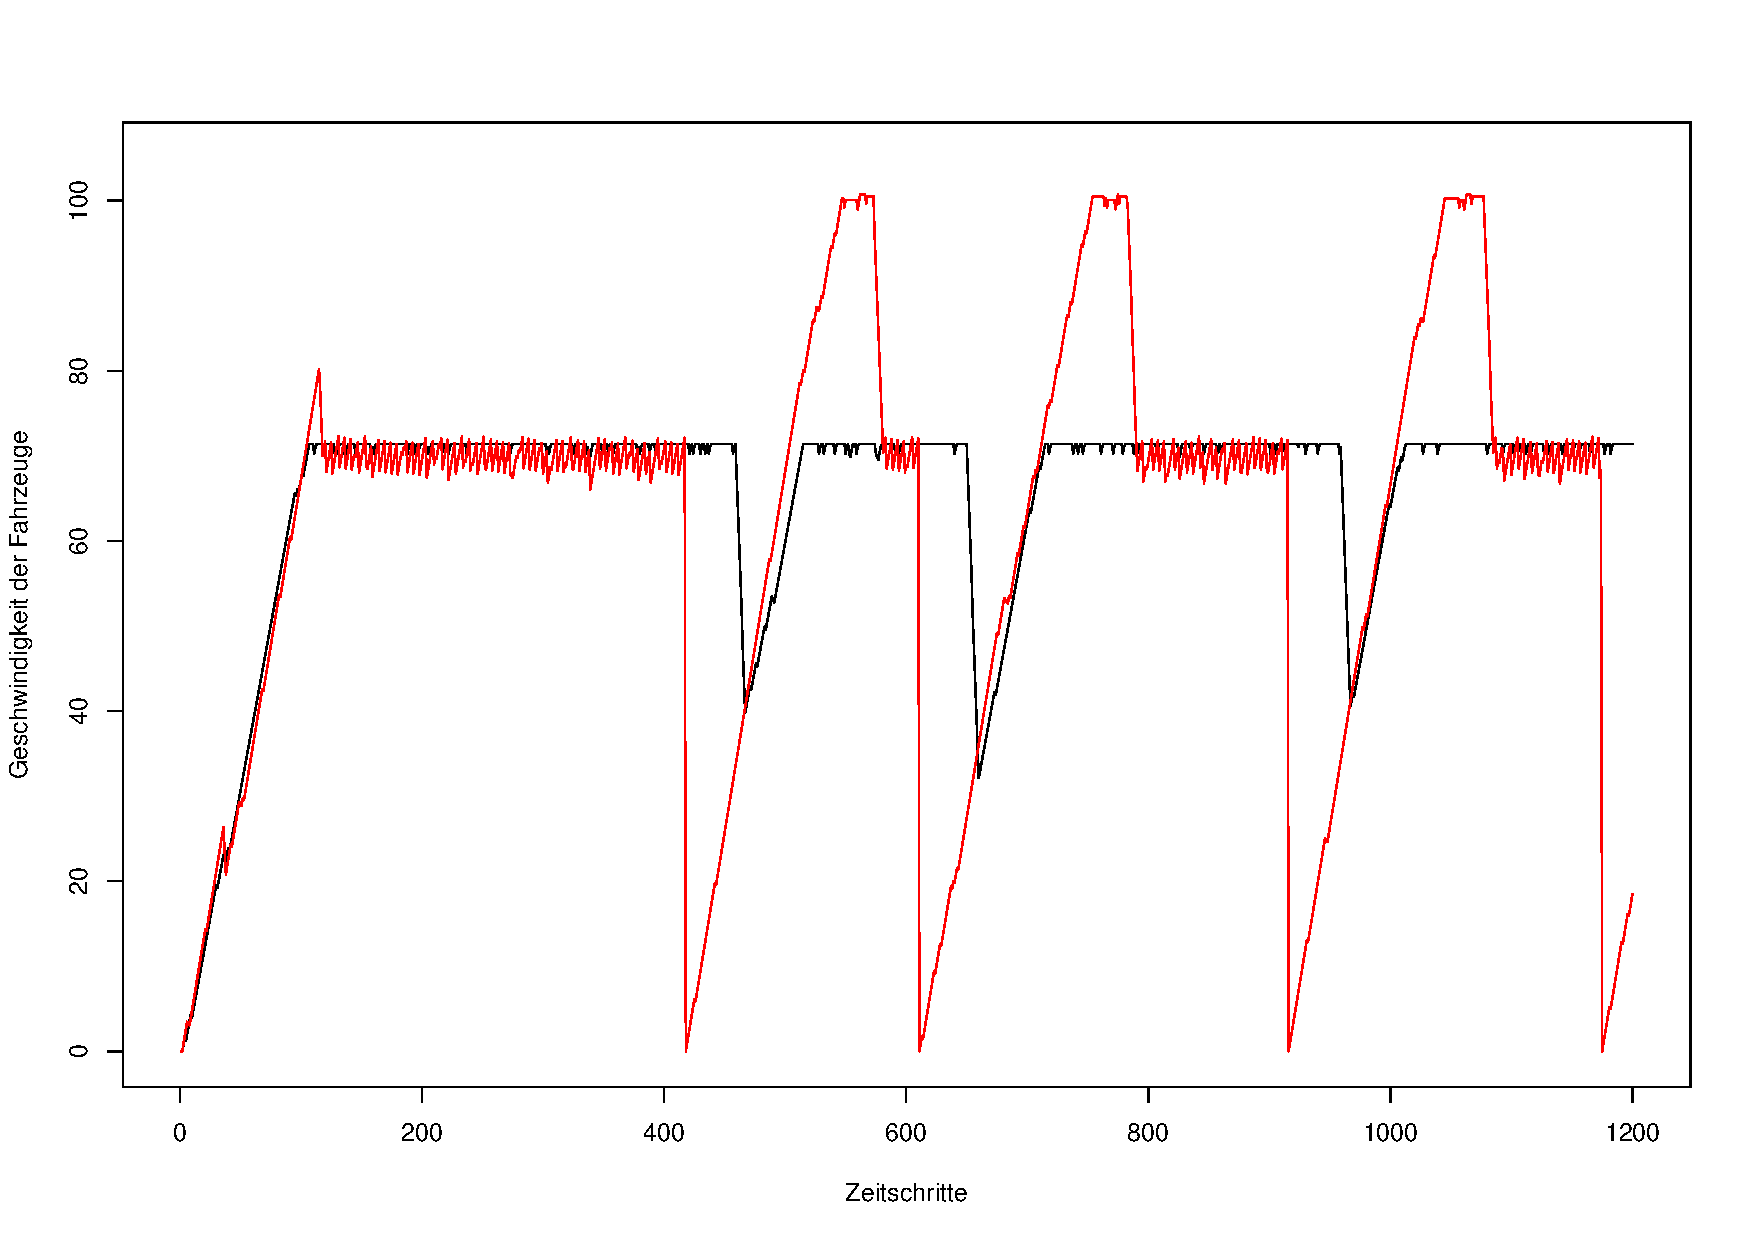
\includegraphics[width=0.3\textwidth]{speed_run19a}\label{figure:run19a}}\qquad 
   \subfigure[Modifikation 1]{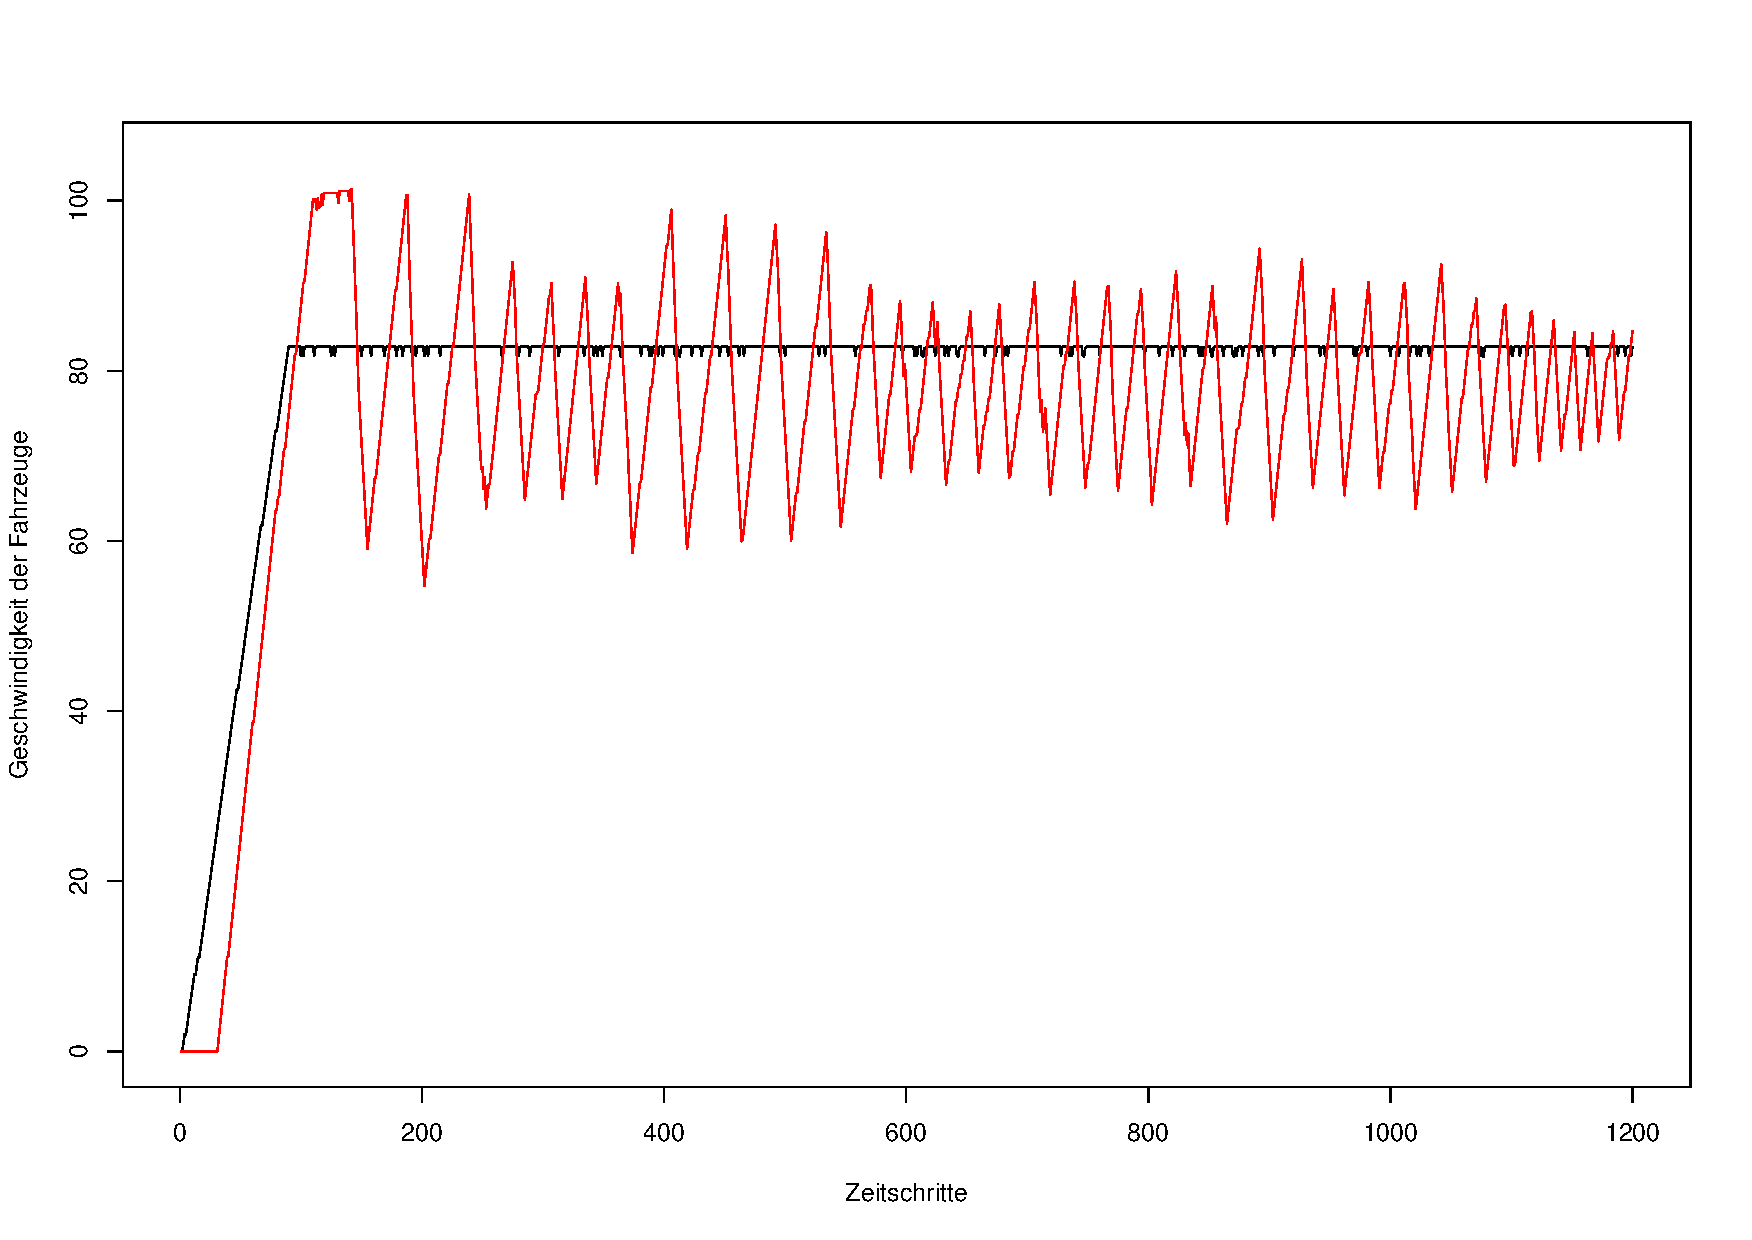
\includegraphics[width=0.3\textwidth]{speed_run19b}\label{figure:run19b}}\qquad 
   \subfigure[Modifikation 2]{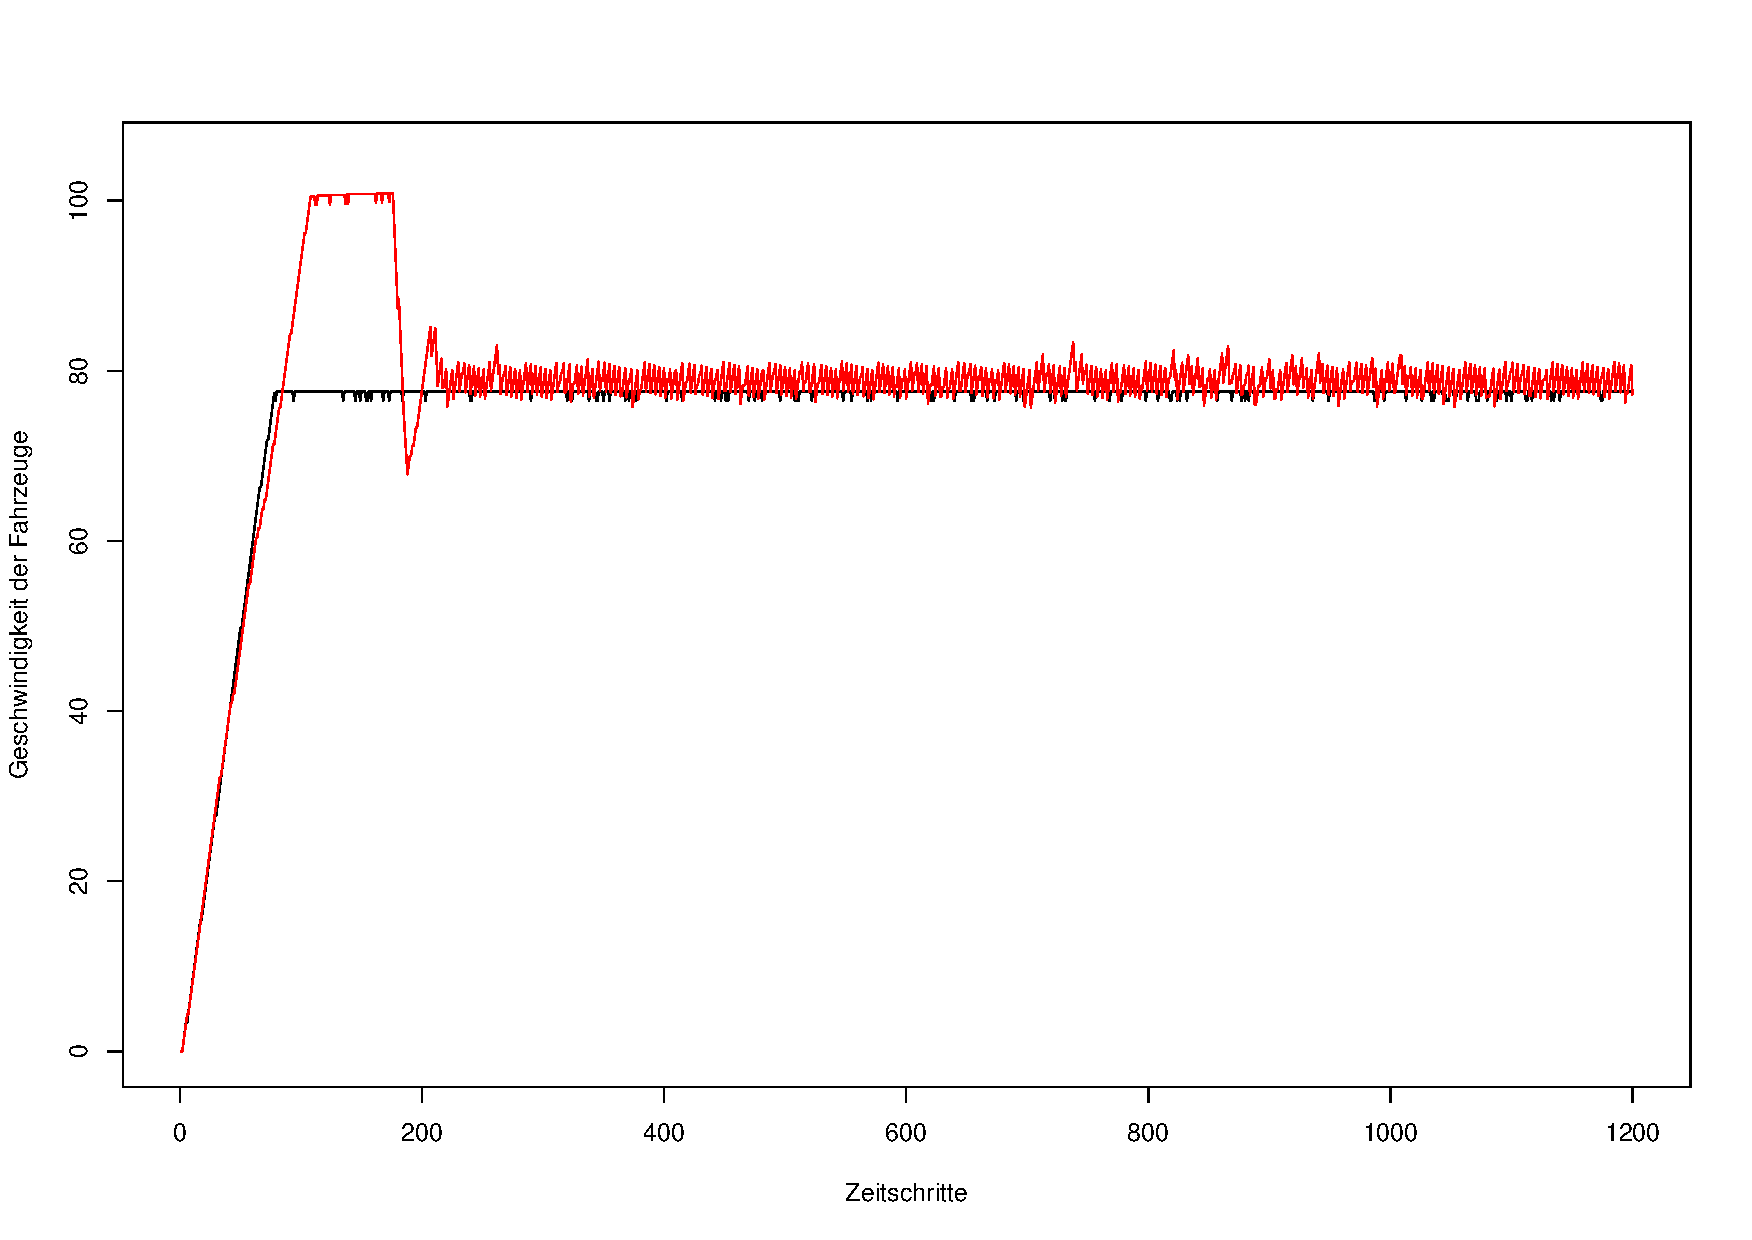
\includegraphics[width=0.3\textwidth]{speed_run19c}\label{figure:run19c}}
  \caption{Simulationen mit Veränderungen in den Agentenplänen} 
  \label{figure:run19a-c}
\end{figure}

Eine erste Modifikation führte wieder zurück zu einem Verhalten, siehe \cref{figure:run19b}, aufgrund dessen die Geschwindigkeitskomponente mit in die Verzögerungslogik eingefügt worden war. 
\\
Das nachfolgende Fahrzeug bremste so lange ab, bis der gewünschte Abstand erreicht war, um daraufhin mit einem \enquote{Zwischensprint} wieder auf das vorausfahrende Fahrzeug aufzuschließen.
Durch den Geschwindigkeitsüberschuss, der abgebaut werden muss, wurde der Abstand wieder extrem verkürzt, dass der Kreis von vorn beginnt.

In einigen Simulationsläufen musste die Geschwindigkeit derart massiv abgebaut werden, dass das Folgefahrzeug zum Stillstand kam.

Es musste ein Weg gefunden werden, die Geschwindigkeit von \enquote{Ego} in Zusammenhang mit der Entfernung vom vorausfahrenden Fahrzeug zu bringen.
\\
Verschiedene Ansätze, bei denen in den Bedingungen der Logik mit den vorliegenden Werten Berechnungen durchzuführen gewesen wären, wurden von der Simulationsplattform nicht unterstützt.
\\
Da den Agenten sowohl die eigene Geschwindigkeit als auch die Entfernung als numerische Werte bekannt sind, werden diese nun zu einander in Beziehung gesetzt.

Dies führt dazu, dass die eigene Geschwindigkeit des betrachteten Fahrzeugs gleichzeitig der jeweilige Mindestabstand vom Vordermann sein muss. 
\\
Eine gleichwertige Bedingung wurde auch für die Simulation der Beschleunigung übernommen.
Der reine Geschwindigkeitsvergleich wurde entfernt.


\subsubsection{Zellgröße 2,5 m}

Aufgrund der Veränderung in den Agentenplänen wurde die erneut verringerte Zellgröße ebenfalls mit den beiden verbliebenen Zeitschrittwerten simuliert.

\begin{figure}[hptb]
  \centering 
   \subfigure[1. Durchlauf]{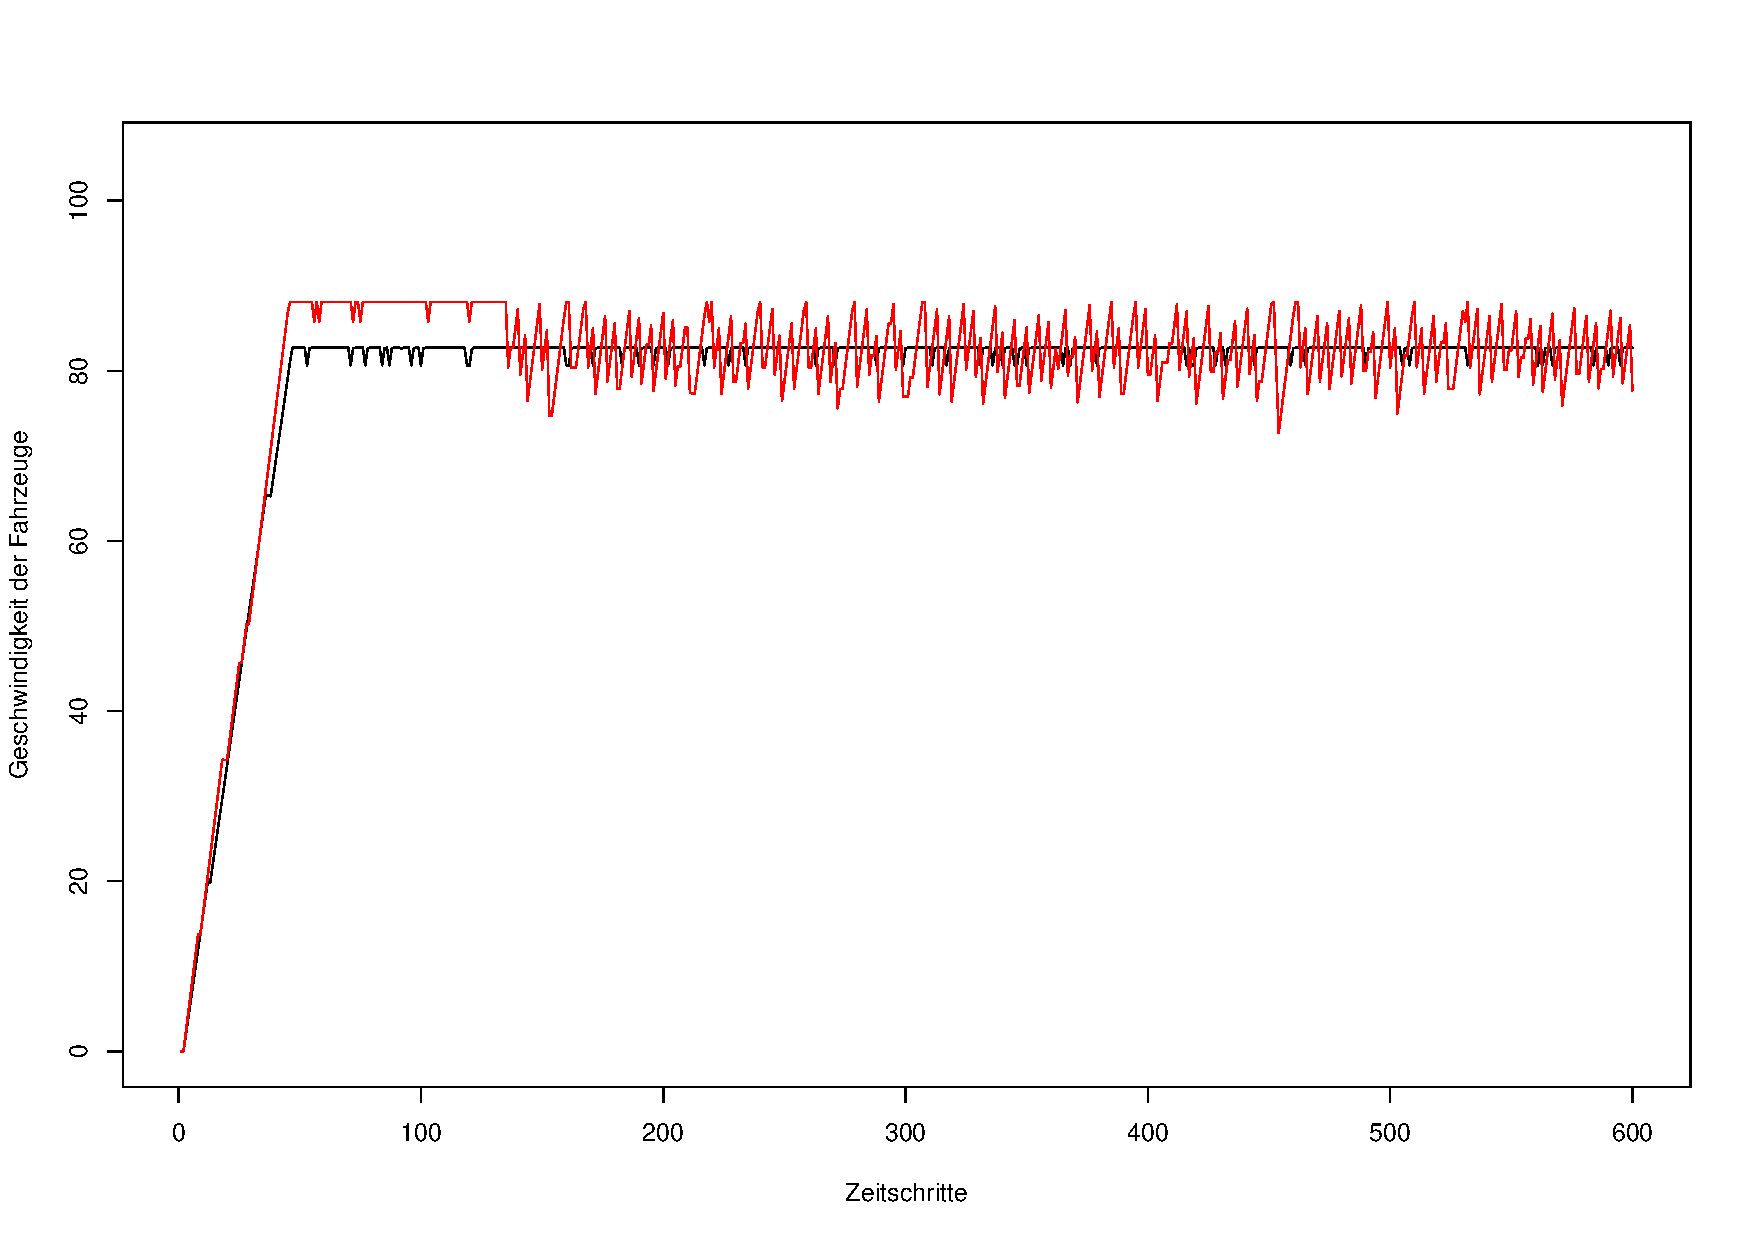
\includegraphics[width=0.3\textwidth]{speed_run24}\label{figure:run24}}\qquad 
   \subfigure[2. Durchlauf]{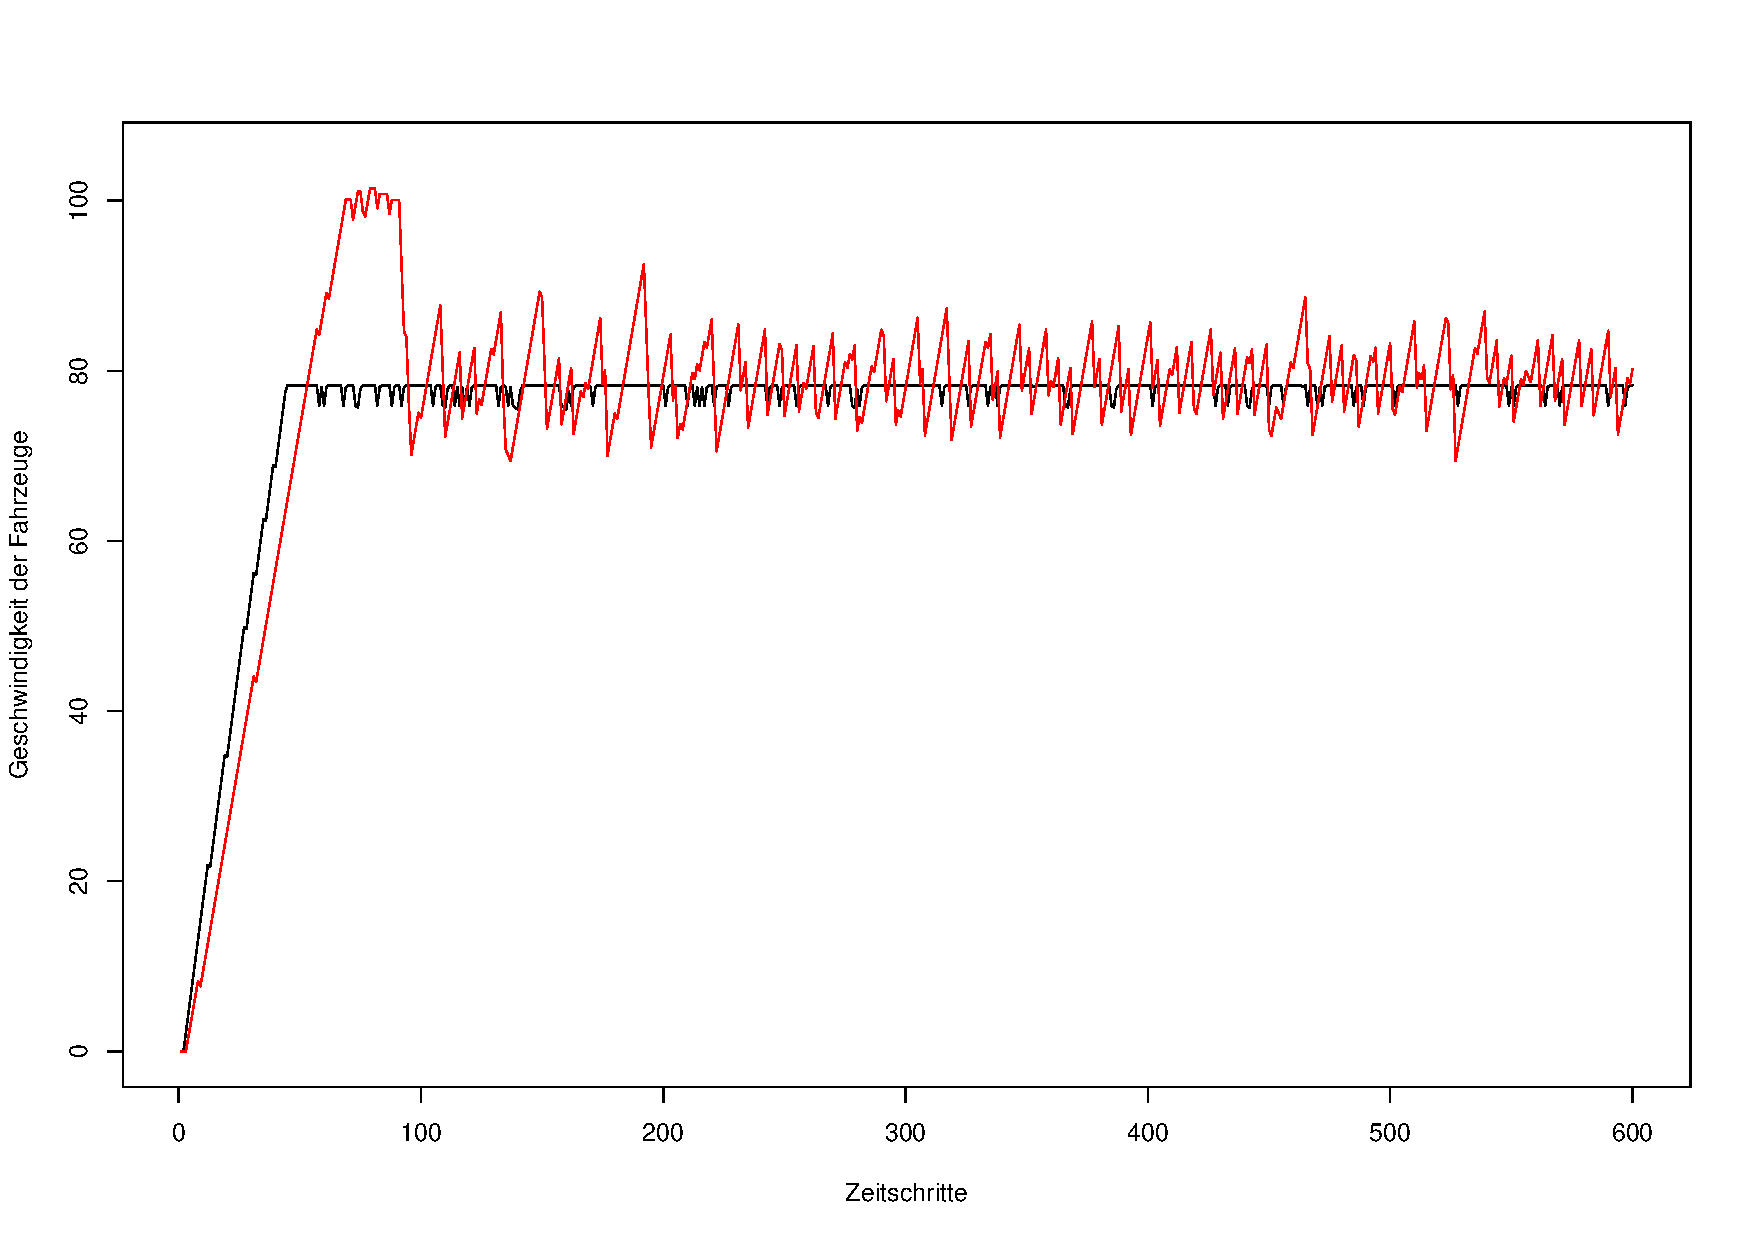
\includegraphics[width=0.3\textwidth]{speed_run25}\label{figure:run25}}\qquad 
   \subfigure[3. Durchlauf]{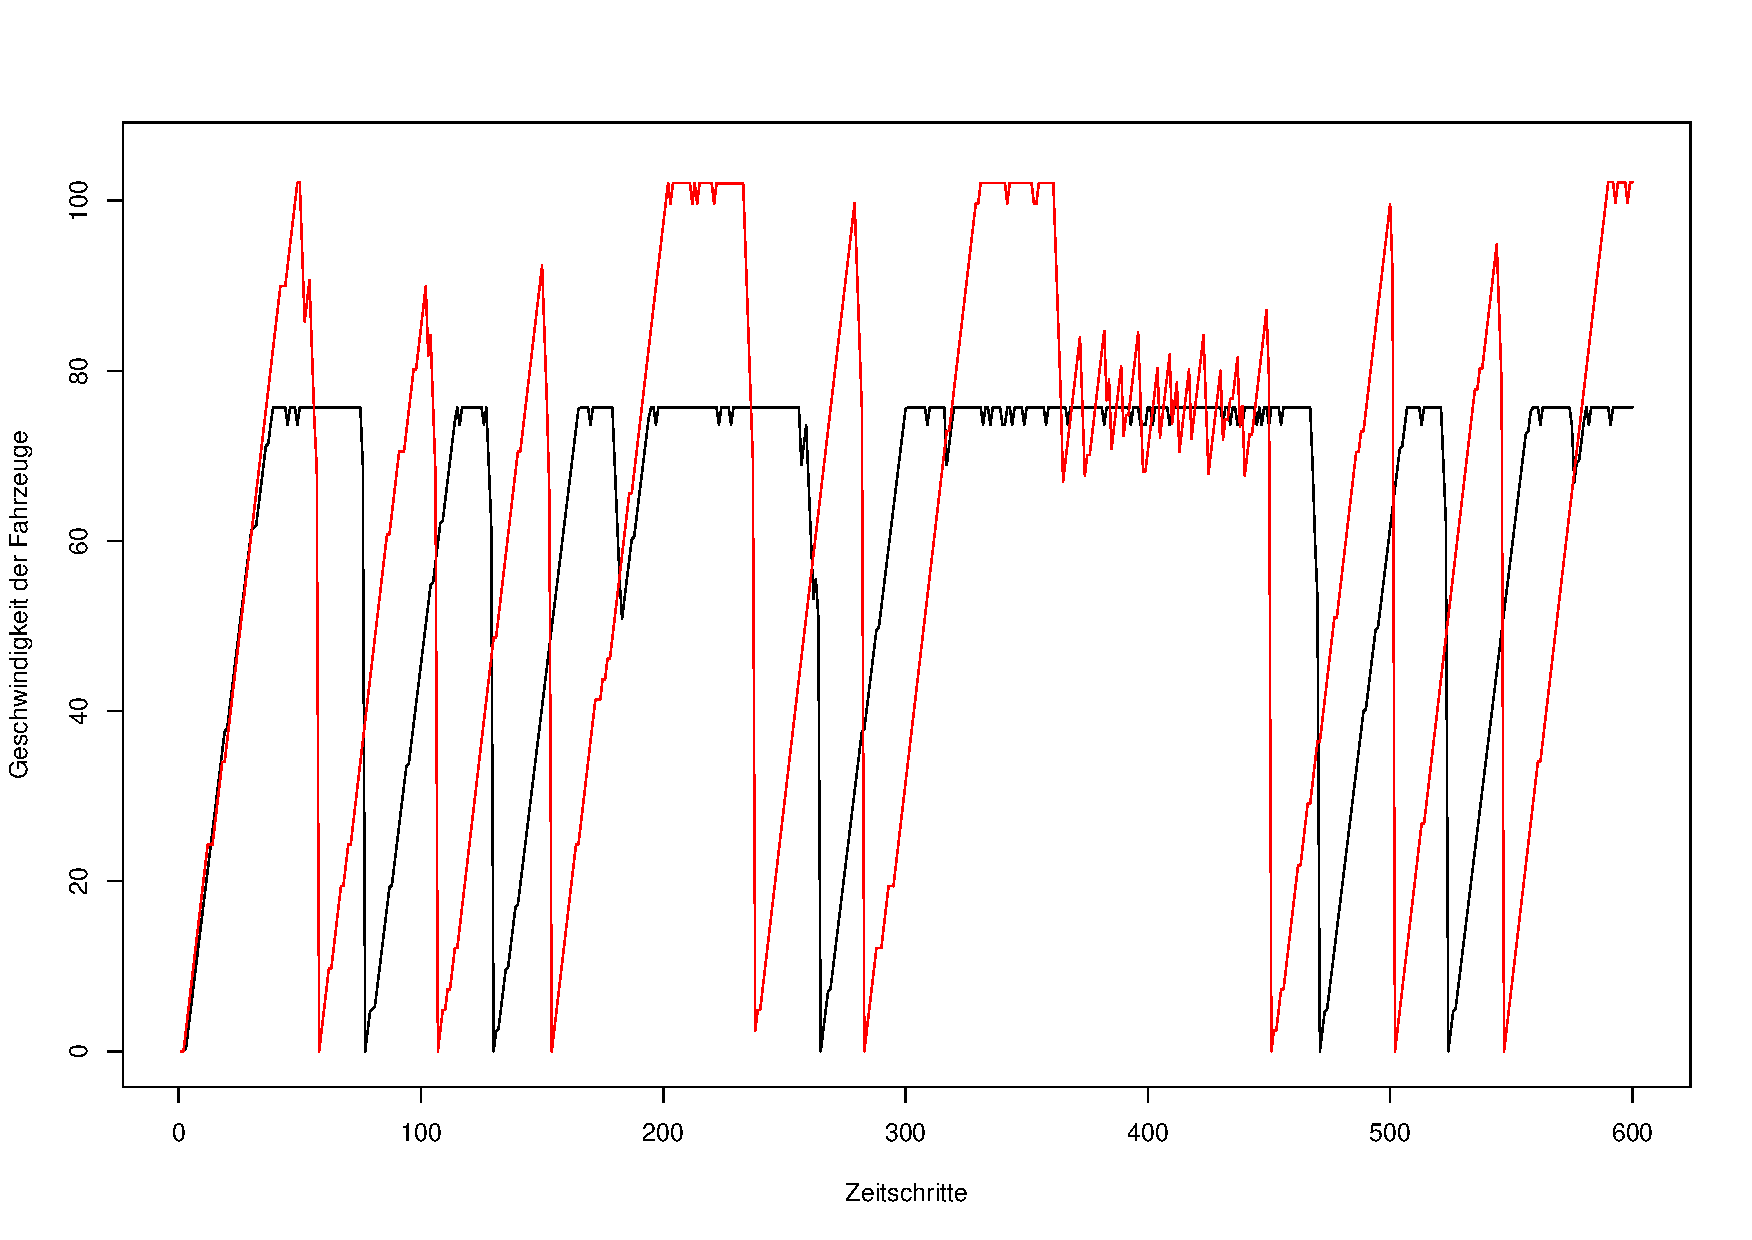
\includegraphics[width=0.3\textwidth]{speed_run26}\label{figure:run26}}
  \caption{Simulationen mit Zellgröße 2,5 m und Zeitschrittlänge 0,05 min} 
  \label{figure:run24-26}
\end{figure}

Die ersten beiden Simulationen mit 2,5 m/0,05 min zeigten ein Bild, welches nach den Veränderungen zu erwarten war.
In der dritten Durchführung traten allerdings wieder Kollisionsereignisse auf.

\begin{figure}[hptb]
  \centering 
   \subfigure[1. Durchlauf]{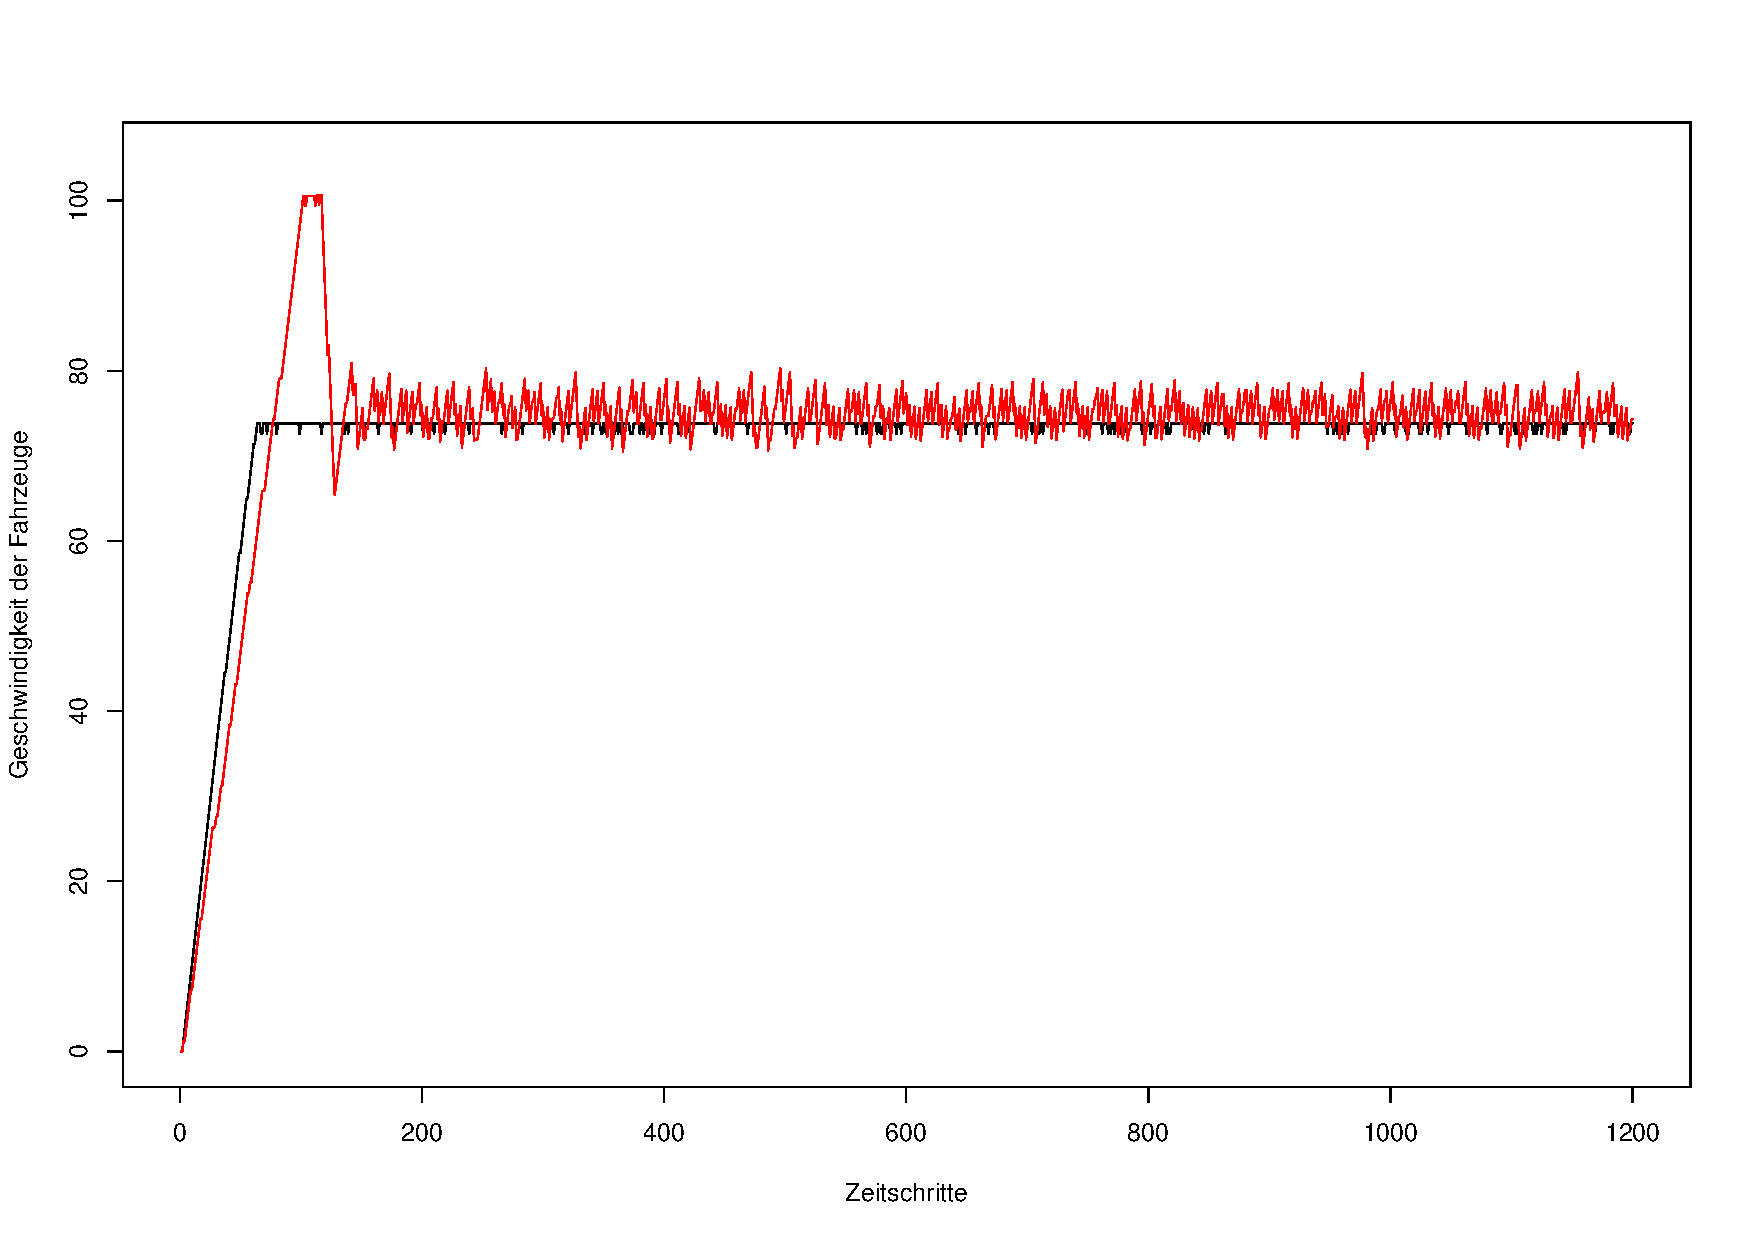
\includegraphics[width=0.3\textwidth]{speed_run27}\label{figure:run27}}\qquad 
   \subfigure[2. Durchlauf]{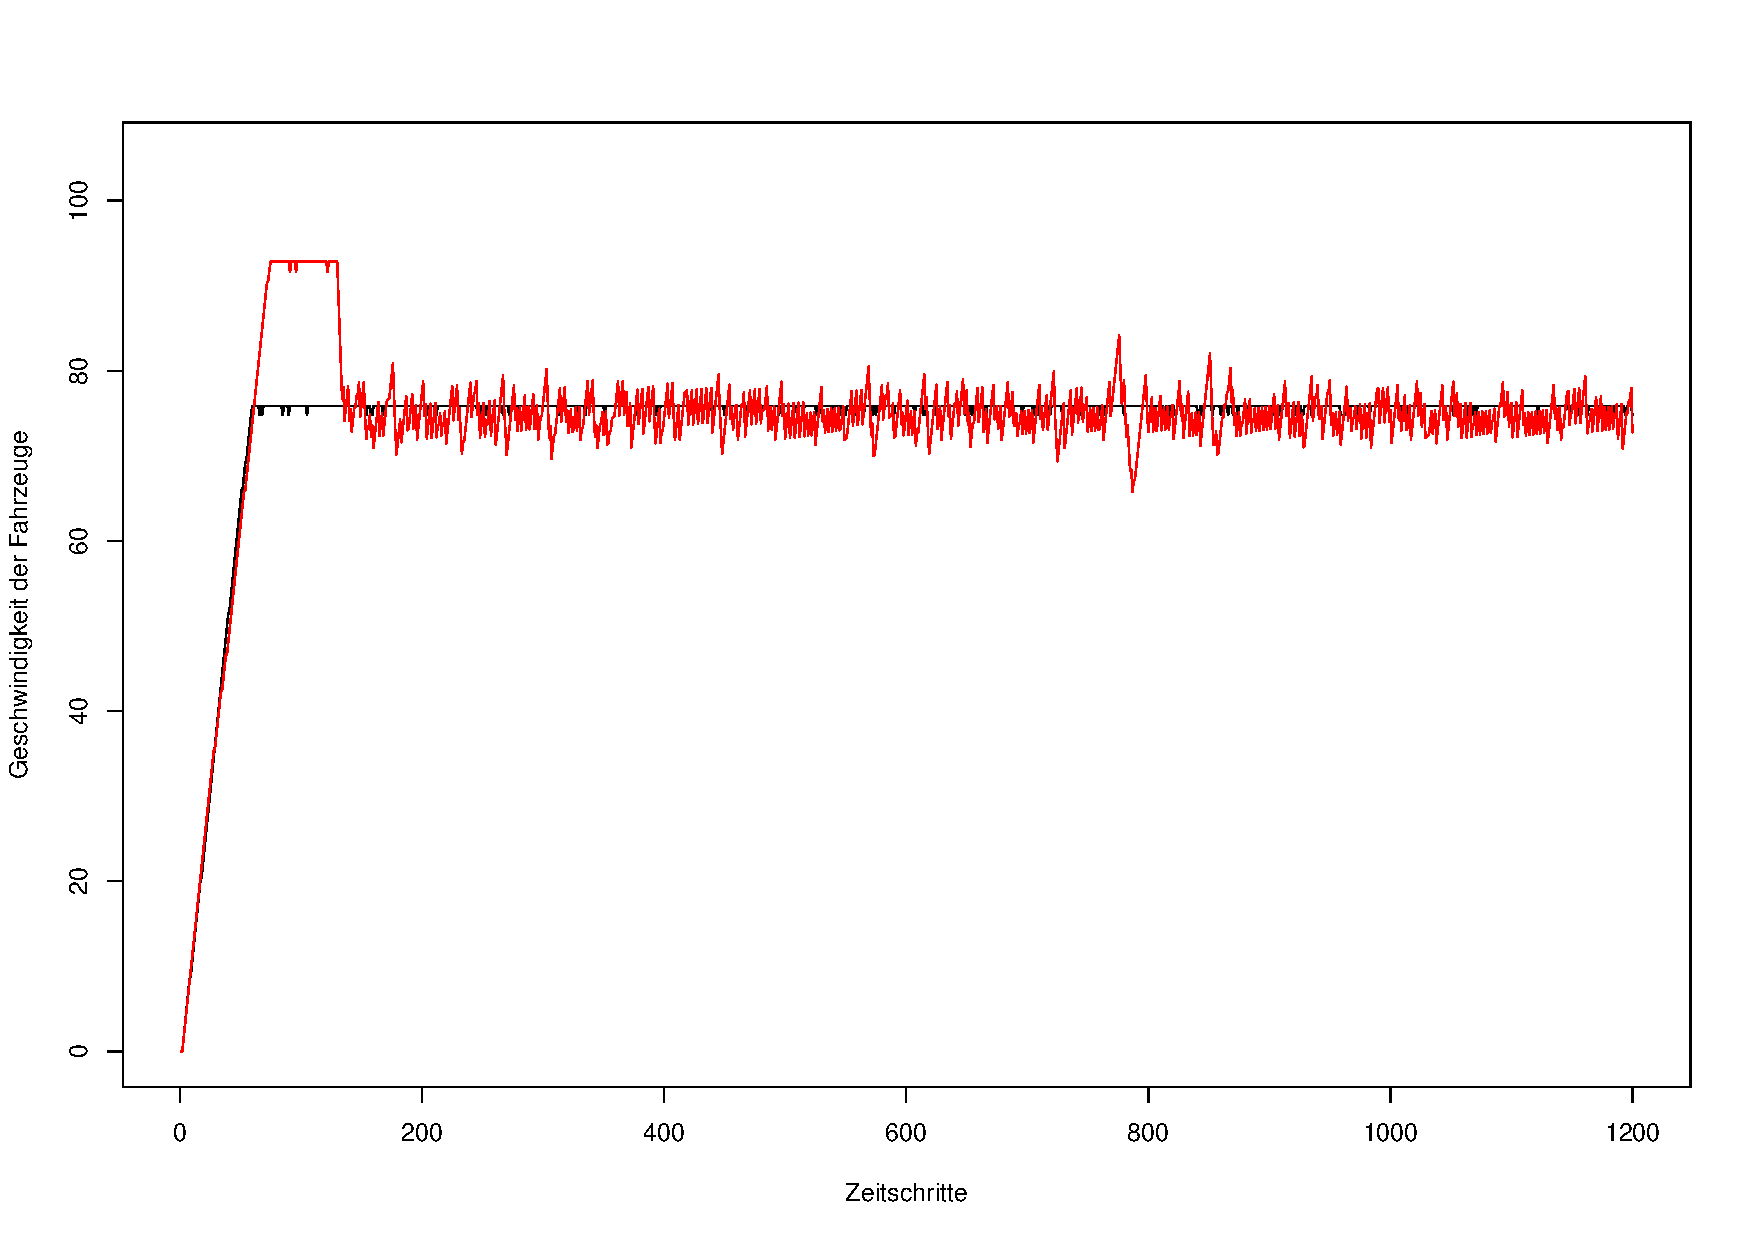
\includegraphics[width=0.3\textwidth]{speed_run28}\label{figure:run28}}\qquad 
   \subfigure[3. Durchlauf]{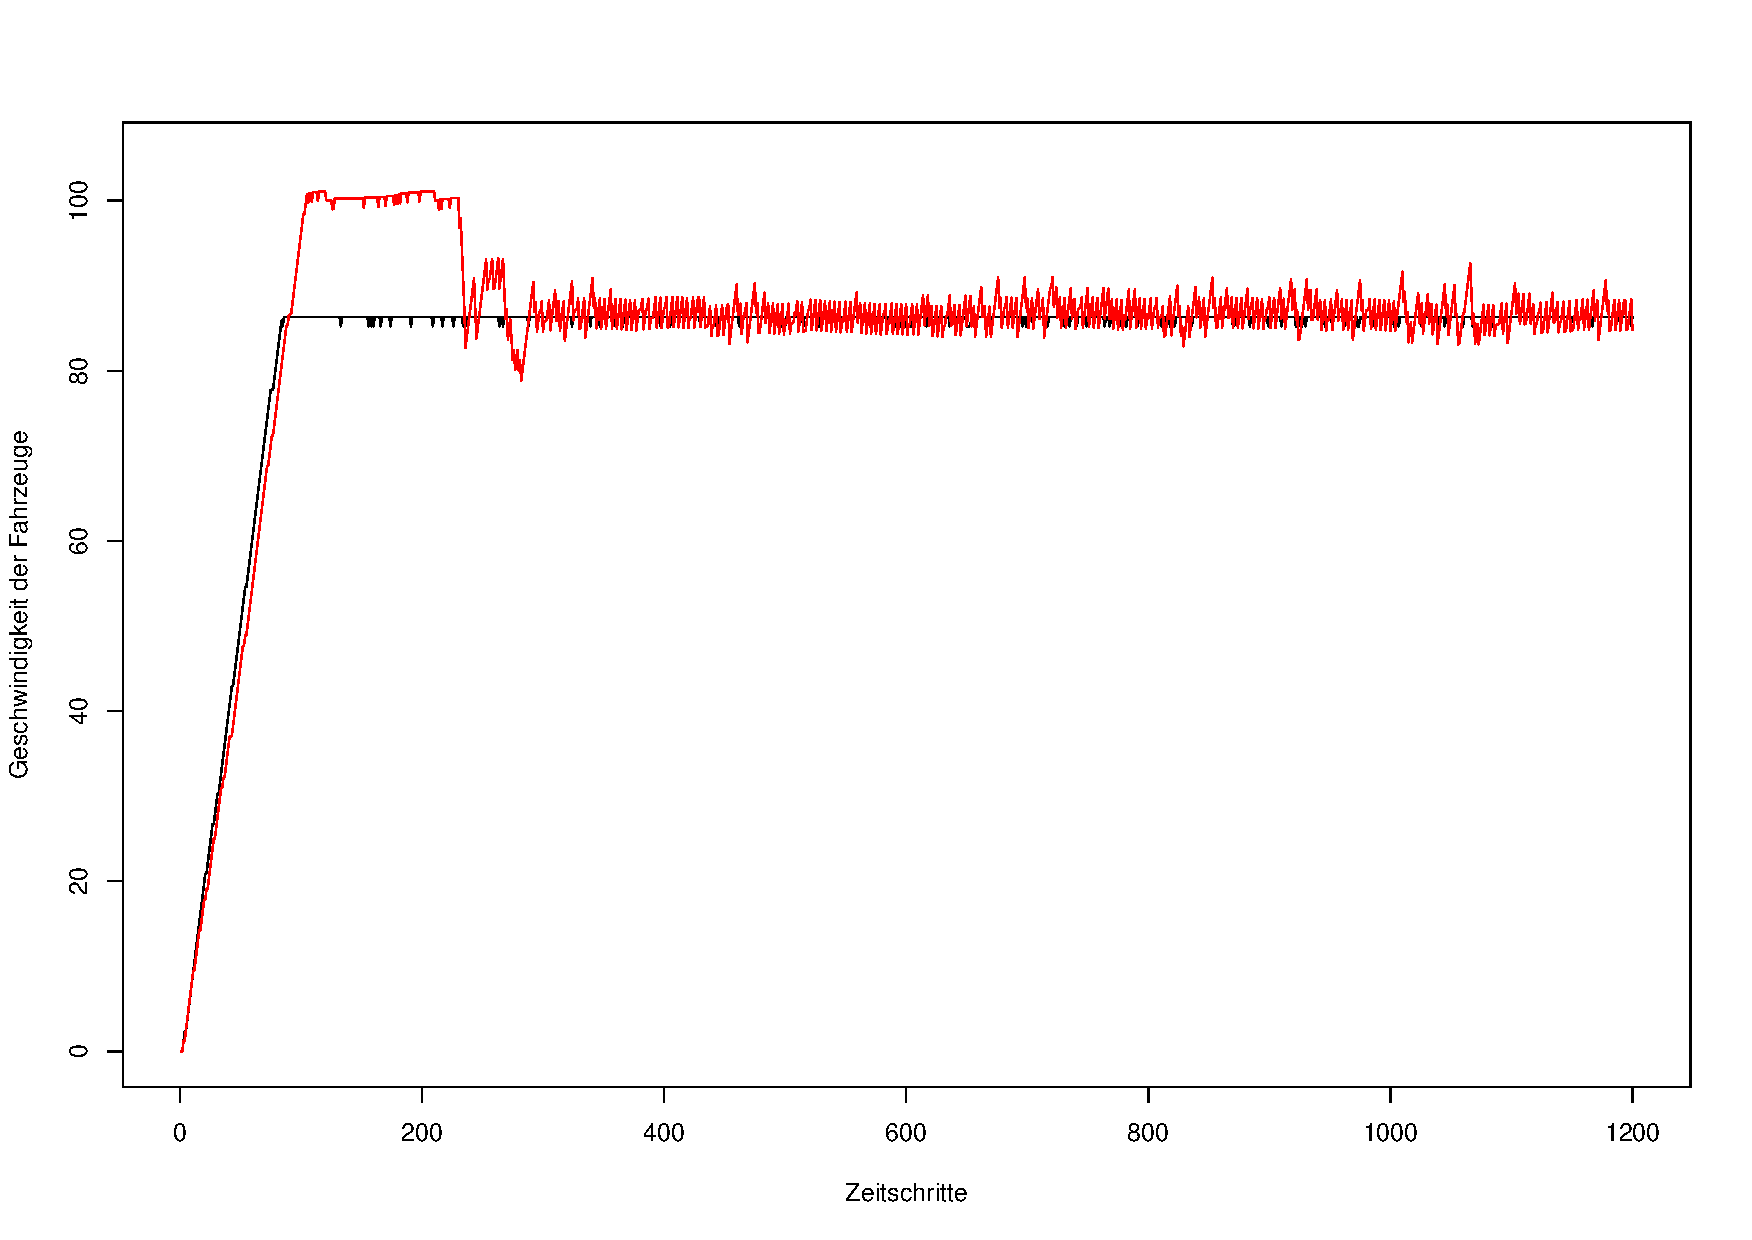
\includegraphics[width=0.3\textwidth]{speed_run29}\label{figure:run29}}
  \caption{Simulationen mit Zellgröße 2,5 m und Zeitschrittlänge 0,025 min} 
  \label{figure:run27-29}
\end{figure}

Die Simulationen der 2,5 m/0,025 min-Variante zeigten [ein sehr gutes Verhalten]\sa{own: anders}.
$Fzg^{S}$ konnte ohne Kollision hinter $Fzg^{L}$ abbremsen und sich dessen Geschwindigkeit anpassen.
\\
Es wurden insgesamt zehn weitere Durchgänge mit diesem Setup durchgeführt. 
Dabei wurde zweimal je eine Kollision beobachtet, die aber immer im Bereich der Beschleunigungsphase am Anfang der Simulation stattfand. 

\subsubsection{\texorpdfstring{Zellgröße $ < $ 2,5 m}%
                              {Zellgröße kleiner als 2,5 m}}

Bei vorhergehenden Testläufen wurde festgestellt, dass es bei einer Zellgröße von weniger als 2,5 Meter zu Inkonsistenzen in den Beliefbases der Agenten kommt.
Entscheidungen müssten dann aufgrund unterschiedlicher Voraussetzungen getroffen werden.
Aus diesem Grund wurde auf den Einsatz von kleineren Zellgrößen verzichtet.
